% http://www.idsc.ethz.ch/education/theses-semester-projects.html
% IDSC LaTeX Thesis Template
% 
% Author(s):	Eric Müller
% 				Institute for Dynamic Systems and Control
% 				Swiss Federal Institute of Technology (ETH) Zurich
% 
% Created:		2004/04/02  (Eric Mueller)
% 
% Notes: Has been tested on Windows 7 + MikTeX + TeXnicCenter
%
% Revisions: 	2009/05/29  (Soren Ebbesen)
% 				    2011/03/22	(Soren Ebbesen)
%             2013/03/08	(Soren Ebbesen)
%             2014/03/13	(Soren Ebbesen)
% ______________________________________________________________________________
\documentclass[11pt,twoside,a4paper,fleqn]{report}

% specifies to what depth sections shall be enumerated
\setcounter{secnumdepth}{5}
%changes the white space padding below figures
%5pt stands for the padding between float elements (figures), the plus 2pt stands for a fixed 2pt (minus would mean optional)
\setlength{\intextsep}{5pt plus 2pt}   % default value 12pt plus 2pt minus 2pt

\usepackage[english,mt]{ethidsc} % Special IDSC styles and commands      	
								 % {german}/english: language of headings, etc.
								 % {st}/bt/mt: {semester}/bachelor/master thesis
								
% for image positioning
\usepackage[export]{adjustbox}
\usepackage{wrapfig}
\usepackage{graphicx}
% defining the bibliography settings
\usepackage[backend=biber, citestyle=authoryear]{biblatex}
\addbibresource{library.bib}
% placing figures next to each other with subfigures
\usepackage{subcaption}
% for displaying code snipplets
\usepackage{listings}
\usepackage{amsmath}
\usepackage{mathtools}
							
% Page header (don't change)____________________________________________________
\setlength{\parindent}{0em}                 % Disable parindent
\rhead[\nouppercase{\rightmark}]{\thepage}  % Special headings
\lhead[\thepage]{\nouppercase{\leftmark}}   % Special headings
\cfoot{}                                    % Special headings


% Title page (please fill in)___________________________________________________
\title{\LaTeX\ Thesis Template v.1.4}


\studentA{Maximilian Hartmann}
\ethidA{13-061-619}
\semesterA{5}
\emailA{hartmanm@student-net.ethz.ch}

%\studentB{Second Student}
%\ethidB{12-345-678}
%\semesterB{9}
%\emailB{second@student.ethz.ch}

%\supervision{Dr. Marcel Hunziker (ETH and WSL)\\ Dr. Flurina Wartmann (WSL)\\ Prof. Dr. Ross Purves (UZH)\\ Dr. Rahul Deb Das (UZH)}
\date{April 2019}

%\identification{IDSC-XX-YY-ZZ} 		% Project identifier

\infopage
\declaration

% Begin document___________________________________________________________

\begin{document}

\maketitle 							% Create title page


% Preamble______________________________________________________________________

\pagenumbering{roman} 				% Begin roman page numbering (i,ii,...)

%---------------------------------------------------------------------------
% Preface
% asterisk signals a title without numbering
%\chapter*{Preface}
%\

%Blah blah \dots

% \clearpage
%---------------------------------------------------------------------------
% Abstract

%\chapter*{Zusammenfassung}
% \addcontentsline{toc}{chapter}{Zusammenfassung}

%Bla bla \dots

\cleardoublepage

\chapter*{Abstract}
 \addcontentsline{toc}{chapter}{Abstract}
Where do people perform Nature-Based Recreation Activities (NBRAs) and what factors draw them to specific areas? Recreation as a form of stress relief has become more important with increased rates of mental illnesses. This thesis fosters the information retrieval related to the recreational usage of space and shall support future planning. Thereby, georeferenced Social Media Data (SMD) of the Social Media Platforms (SMPs) Instagram and Flickr is used to predict the occurrences of seven distinct NBRA-classes in the research area located inside the Canton of Zug, Switzerland. 'Walking', 'hiking', 'jogging', 'biking', 'dog walking', 'horse riding' and 'picnicking' are the considered classes. \\
Machine Learning (ML) in combination with the deep-learning image recognition algorithm \textit{Google Cloud Vision} - that extracts labelled image elements - was used to train two text-classification models to identify the seven NBRA-classes inside Instagram and Flickr media objects (posts). Many models of previous scientific studies either drew upon the text or image contained information but rarely were these two data-sources used in conjunction. One focal point of this thesis investigates the effect of training a model on a combination of text-data and image-data to potentially achieve an improved model performance. The linear Support Vector Classifier (linearSVC) and the decision tree based Random Forest fitting algorithm were tested. This approach functions as a complement to conventional data-acquisition methods such as surveys and interviews but with the benefits of potentially higher spatial and temporal resolutions as well as a cheaper implementation. Ground truth data in the form of passive observations of NBRAs and 52 interviews was additionally acquired in three locations of the research area. This data was used on one hand to justify the legitimacy of the created models and on the other hand to acquire behavioural and demographic information about the social media presence of the interviewees. Finally, Foursquare data was used to evaluate the allocation efficiency of existing recreation related infrastructure compared to the peoples' usage of space derived from the SMD.\\
The results revealed a slightly higher performance for the linearSVC model trained on text as well as image-data with a manually verified average precision of 0.749 across all classes on unseen Instagram and Flickr data. The major improvement however lies in the achievement of twice as many correctly classified media objects containing NBRAs than compared to the model that was solely trained on text-data. Therefore, a recall and generalisation increase were recorded. No significant precision difference was detected for predictions on media objects from different SMPs.
The model outputs enabled the creation of maps which show the spatial distribution of the seven NBRA-classes in the research area. \\
\newline
\textbf{Keywords:} recreation activities, text-classification model, image recognition, social media data

\cleardoublepage

\chapter*{Acknowledgements} \label{acknowledgements}
  \addcontentsline{toc}{chapter}{Acknowledgements}
I would like to express my very great appreciation to all my supervisors, friends and institutions that helped me during the course of this thesis. First of all I want to thank ETH for providing me with the infrastructure, research literature and needed resources that allowed the start and completion of this thesis.\\
Personally I want to sincerely thank Dr. Marcel Hunziker for approving my master thesis proposal that originated from a term paper of the 'Advanced Landscape Research' lecture which he also supervised. \\
I would like to offer my special thanks to Dr. Flurina Wartmann from the WSL who was my primary contact throughout the entire thesis and who assisted me in setting up the ground truthing as well as in various administrative concerns. \\
Prof. Dr. Ross Purves and Dr. Rahul Deb Das from the geocomputation unit of the University of Zurich provided me with expert knowledge in all programming related issues for which I am deeply grateful.\\
\newline
Additionally, I would like to thank the spatial planing department of the Canton of Zug - especially Martina Brennecke and Alexander Gnos. Former for her personal assistance and insight on relevant projects in the research area and latter for his provision of needed geo-data in the form of shapefiles. My special thanks are extended to the staff of the company Zugerbergbahn, particularly to Christoph Sidler for providing me with passenger numbers of their mountain railway. \\
\newline
I cannot thank my sister Florence enough for conducting the entire 'passive observation' - an essential part of the ground truthing. This part would not have been possible without her. And finally I want to thank and mention my friends Achilleas Lehmann and Christopher O'Bryan who proofread my thesis and gave constructive feedback that lead to this final version of my thesis.

\cleardoublepage
%---------------------------------------------------------------------------
% Table of contents

 \setcounter{tocdepth}{2}
 \tableofcontents
 \listoftables\addcontentsline{toc}{chapter}{List of Tables}
 \listoffigures\addcontentsline{toc}{chapter}{List of Figures}

 \clearpage

%---------------------------------------------------------------------------
% Symbols

\chapter*{Nomenclature}\label{chap:symbole}
 \addcontentsline{toc}{chapter}{Nomenclature}

%\section*{Symbols}
%\begin{tabbing}
% \hspace*{1.6cm} \= \hspace*{8cm} \= \kill
% $\mathrm{EHC}$ \> Conditional equation \> [$-$] \\[0.5ex]
% $e$ \> Willans coefficient \> [$-$] \\[0.5ex]
% $F,G$ \> Parts of the system equation \> [\unitfrac[]{K}{s}]
%\end{tabbing}

%\section*{Indicies}
%\begin{tabbing}
% \hspace*{1.6cm}  \= \kill
% a \> Ambient \\[0.5ex]
% air \> Air
%\end{tabbing}

\section*{Acronyms and Abbreviations}
\begin{tabbing}
 \hspace*{1.6cm}  \= \kill
 API \> Application Program Interface \\
 CSV \> Comma Separated Values \\
 ES \> Ecosystem Services \\
 ETH \> Eidgen\"{o}ssische Technische Hochschule \\
 GIS \> Geographical Information System \\
 GPS \> Global Positioning System \\
 GUI \> Graphical User Interface \\
 HTML \> Hypertext Markup Language \\
 IR \> Information retrieval \\
 JSON \> JavaScript Object Notation \\
 M1 \> Machine learning model NR.1 that was trained on text-data \\
 M2 \> Machine learning model NR.2 that was trained on text-data and image-data \\
 ML \> Machine Learning \\
 NBRA \> Nature-based Recreation Activity \\
 NLTK \> Natural Language processing Toolkit \\ 
 RDBMS \> Relational Database Management Systems \\
 SMD \> Social Media Data \\
 SMP \> Social Media Platform \\
 SVM \> Support Vector Machine \\
 SVC \> Support Vector Classifier \\
 SQL \> Structured Query Language \\
 TF-IDF \> Term Frequency times Inverse Document Frequency \\
 TOS \> Terms of Service \\
 UGC \> User Generated Content \\
 URL \> Uniform Resource Locator \\ 
 VGI \> Volunteered Geographic Information
\end{tabbing}

\section*{Definitions} \label{definitions}
% hspace*{1.6cm}  \= \kill
\texttt{API:} Application interfaces allow the controlled access of programs to specific services of a software system. 
\newline

\texttt{API endpoint:} Describes a specific service or communication channel a user can access to interact with an API. Different API endpoints provide the user with different data.
\newline

\texttt{Bulk upload:} In the context of this thesis, bulk uploads describe a certain amount of simultaneously or during a short period of time uploaded media objects to the same social media platform by a single author.
\newline

\texttt{Feature/word-token/token:} All these terms describe the features of a text-classification model and have identical meaning in the context of this thesis.
\newline

\texttt{Media object:} All user generated social media data that has been acquired through a API or third party company will be referred to as media objects. In the sense of machine learning the term media object can be used interchangeably with the term 'document'.
\newline

\texttt{Netlytic:} A third party company which provides licensed data of numerous social media platforms (among others Instagram) based on user specific queries.
\newline

\texttt{Pipelining:} Sequence of functions where the output of the preceding function is used as input for the successive function.

\texttt{Regular expression:} A sequence of characters that are used in programming to define string patterns are referred to as regular expressions or also 'regex'.

\cleardoublepage

%---------------------------------------------------------------------------


% Chapters______________________________________________________________________

\pagestyle{fancy}               	% Fancy headings
\pagenumbering{arabic}				% Begin arabic page numbering (1,2,...)

\chapter{Introduction}
\section{Motivation}
The world wide web is a phenomenon of ever increasing dimension and integration into people's lives. In the beginning of 2019 roughly 4.3 Billion people had access to the internet which accounts for 56\% of the entire world population\footnote{https://www.internetworldstats.com/stats.htm\#links, accessed: 30.03.2019}. 
With more people being interconnected the amount of available data simultaneously increases. \\
This data consists of a broad spectrum of information people publicly or unintentionally share on the internet or more specifically among others through web-searches, blogs, chats, video games, online shops and social media platforms (SMP). SMPs provide services which allow users to create an online identity to present themselves to others by sharing personalised information. There are various SMP-providers available such as Facebook, Instagram or Twitter to name a few - all with their specific target audience and descriptive upload content. This social media data (SMD) is referred to as User Generated Content (UGC) or if it is georeferenced as Volunteered Geographic Information (VGI). VGI encompasses people's interests, performed activities, future intentions, sense-of-place and perception of locations \parencite{Goodchild2007}. This geotagged information as it is also known allows for spatial mapping of data in space.  
According to the Federal Statistical Office (FSO) of Switzerland 73\% of people between the age of 16 and 74 were in the year 2017 in the possession of a smart mobile device\footnote{https://www.bfs.admin.ch/bfs/de/home/statistiken/kultur-medien-informationsgesellschaft-sport/informationsgesellschaft/gesamtindikatoren/haushalte-bevoelkerung/mobile-internetnutzung.html, accessed: 30.03.2019}. These devices are generally equipped with the Global Positioning System (GPS) which supports the provision of VGI.
This social media derived big-data holds a lot of potential for various research applications as already highlighted by papers such as \textcite{DiMinin2015, DiMinin2017, Meentemeyer2016}. The main advantages to conventional methods such as surveys and interviews are comparably fast, (mostly) easy and low-priced continuous data-streams as well as a good spatial and temporal coverage at multiple scales.\\
\newline
Also a phenomenon of modern times are increased rates of job induced mental fatigue, stress and illness which are side products of an ever more specialised and demanding economy. To address that issue the report of mental health in Switzerland \parencite{Ruesch2003} was conducted among others by the Federal Office for Public Health (FOPH) which highlights the lack of prevention measures in place. This led to a monitoring program to foster mental health provision and awareness in Switzerland \parencite{Schuler2012} also on a cantonal level. The environment is known to be a sustainable source for mental health benefits by providing a diverse range of recreation possibilities. The extent and potential value associated with these provided ecosystem-services was noted in the 'effects of the environment on human health' report \parencite{Ragettli2017} of the Federal Office for the Environment (FOEN). \\

\section{Problem statement and aim}
Identifying and mapping activities related to nature-based recreation, outdoor recreation or soft ecotourism as described by \textcite{Deng2002, Balmford2009} is the aim of this thesis.
Increasing the quality, quantity and attractiveness of nature-based recreation requires knowledge over the current usage of space. More specifically, in regards to the activities people perform in the environment to answer the following questions: (1) What nature-based recreation activity (NBRA) should be promoted in a certain area and (2) what kind of supportive infrastructure should be constructed to maximise its utilisation? This thesis tries to respond to that current need for information by investigating the potential of SMD in particular from the SMPs Instagram\footnote{https://www.instagram.com/} and Flickr\footnote{https://www.flickr.com/} for analysing and monitoring the spatial occurrences of NBRAs including walking, hiking, jogging, biking, dog walking, horse riding and picnicking in the Canton of Zug, Switzerland. The mentioned SMPs are known for hosting geotagged images with attached user-generated text (for more detailed information refer to section \ref{data_acquisition}) and were proven to be good indicators for multiple applications such as determining visitation rates to nature reserves \parencite{Tenkanen2017, Heikinheimo2017, Keeler2015, Wood2013} or to social events \parencite{Pettersson2011}, human mobility patterns \parencite{Barchiesi2015, Grossenbacher2014} and recreation locations \parencite{Weyland2014, Hill2006, Neuvonen2010}.
Accordingly, this study tries to evaluate the potential of SMD as a proxy for predicting the occurrences of NBRAs as an alternative to conventional data-acquisition methods such as surveys is investigated.\\
The goal of achieving a comparison between the people's usage of space and the already present infrastructure to evaluate an efficient asset allocation was performed with the data of the web-application Foursquare\footnote{https://de.foursquare.com/}. This data consists of categorised infrastructural elements also known as \textit{venues} which were used as indicator for the current dispersion of sport and recreation facilities in the research area. The results of this comparison aim to improve spatial planing by optimising the allocation of recreational infrastructure in correspondence to the where people actually perform certain NBRAs.

\section{Approach}
The approach presented in this thesis creates and evaluates two machine learning (ML) models to predict NBRAs in georeferenced Instagram and Flickr posts. These posts are referred to as media objects throughout the thesis. The first model is trained on a combination of text and image data which has not in this way been done before. The second model was solely trained on text data and functions as a baseline reference to investigate the effect of including image content information. Structural image elements are extracted with the help of a deep-learning algorithm named Google Cloud Vision as also used by \textcite{Richards2018}. The models are individually trained on 1'046 manually classified Instagram media objects originating from a dataset of the region of Zurich \parencite{Gruzd2016} and tuned for best performance. Classification specific model evaluations are subsequently manually conducted on the NBRA-predictions in the research area located in the canton of Zug to compare the two finalised model performances based on untrained data. The innovation of this approach lies in the fully automated prediction process without any manual content analysis which uses dominantly openly accessible and free software. This shall pave the way for a feasible reconstruction and application by e.g. municipal authorities or agencies with a low budget for high priced software licences. \\
\newline
In the course of this thesis, additional ground truth data from interviews and passive observations was acquired in three locations of the research area. The interviews were used to gain insight on three topics. Firstly the drivers that motivate people to visit certain locations above others. Secondly the social media usage of the interviewees in terms of SMP-engagement, upload-frequency and behaviour. Lastly some personal details were recorded which were kept anonymous to gain information about the demographics of social media users. The passive observation as second part of the ground truth was used to count NBRAs-occurrences during the time the interviews were held. In the end the ground truth derived signals were compared to the SMD to evaluate and justify the ML models legitimacy.


\section{Background of machine learning}
This section is laid out to give the reader a short introduction into the field of machine learning (ML) as well as a basic understanding of associated terminologies to help comprehend the applied approach of this thesis.\\
ML in its core refers to the process of a computer to understand or 'learn' the relationships inside a dataset with the help of algorithms to be able to make predictions on data the model has never seen before.
The training's data normally consists of different features which identify and characterise a given entry. The constellation of feature-values which can be metaphorical seen as a 'fingerprint' of a given data point are the reason why a model can potentially make out patterns and relate them to a certain output. This output can either be a class (in the case of a classification problem) or a continuous number (in the case of a regression problem) of new data point.
An example of potential features of a regression problem could be different body measurements of a specific animal with the aim to differentiate between different types of the same species. The training's data would then consist of multiple entries where most likely a human measured the needed body parts of several individuals and entered the continuous numerical value in the corresponding feature field.\\
\newline
One can differentiate between two types of ML - supervised and unsupervised learning. To illustrate the difference imagine a set of training's data where each entry is represented by a point in an n-dimensional space where \textit{n} corresponds to the number of features present and the coordinates of each point (position vector of that point) correspond to the feature's values. If we make the link back to the example above then unsupervised learning would mean that the training's data consists of only the training's data without any labels. The labels in this case would have been the names of the animal species that the measurements were taken from. In this way the model is forced to find natural breaks / boundaries on its own in the training's data by clustering similar data points together and regarding them as an independent class. The hypothesis here is that points closer to each other in space are more related to one another than distant ones - similar to the first law of geography. These model given class names do not correspond in any way to the actual names of the animals because the model has no information on it what so ever. It is up to the user to appropriately label the clusters / classes the model isolated.

\begin{figure}[h]
   \centering
   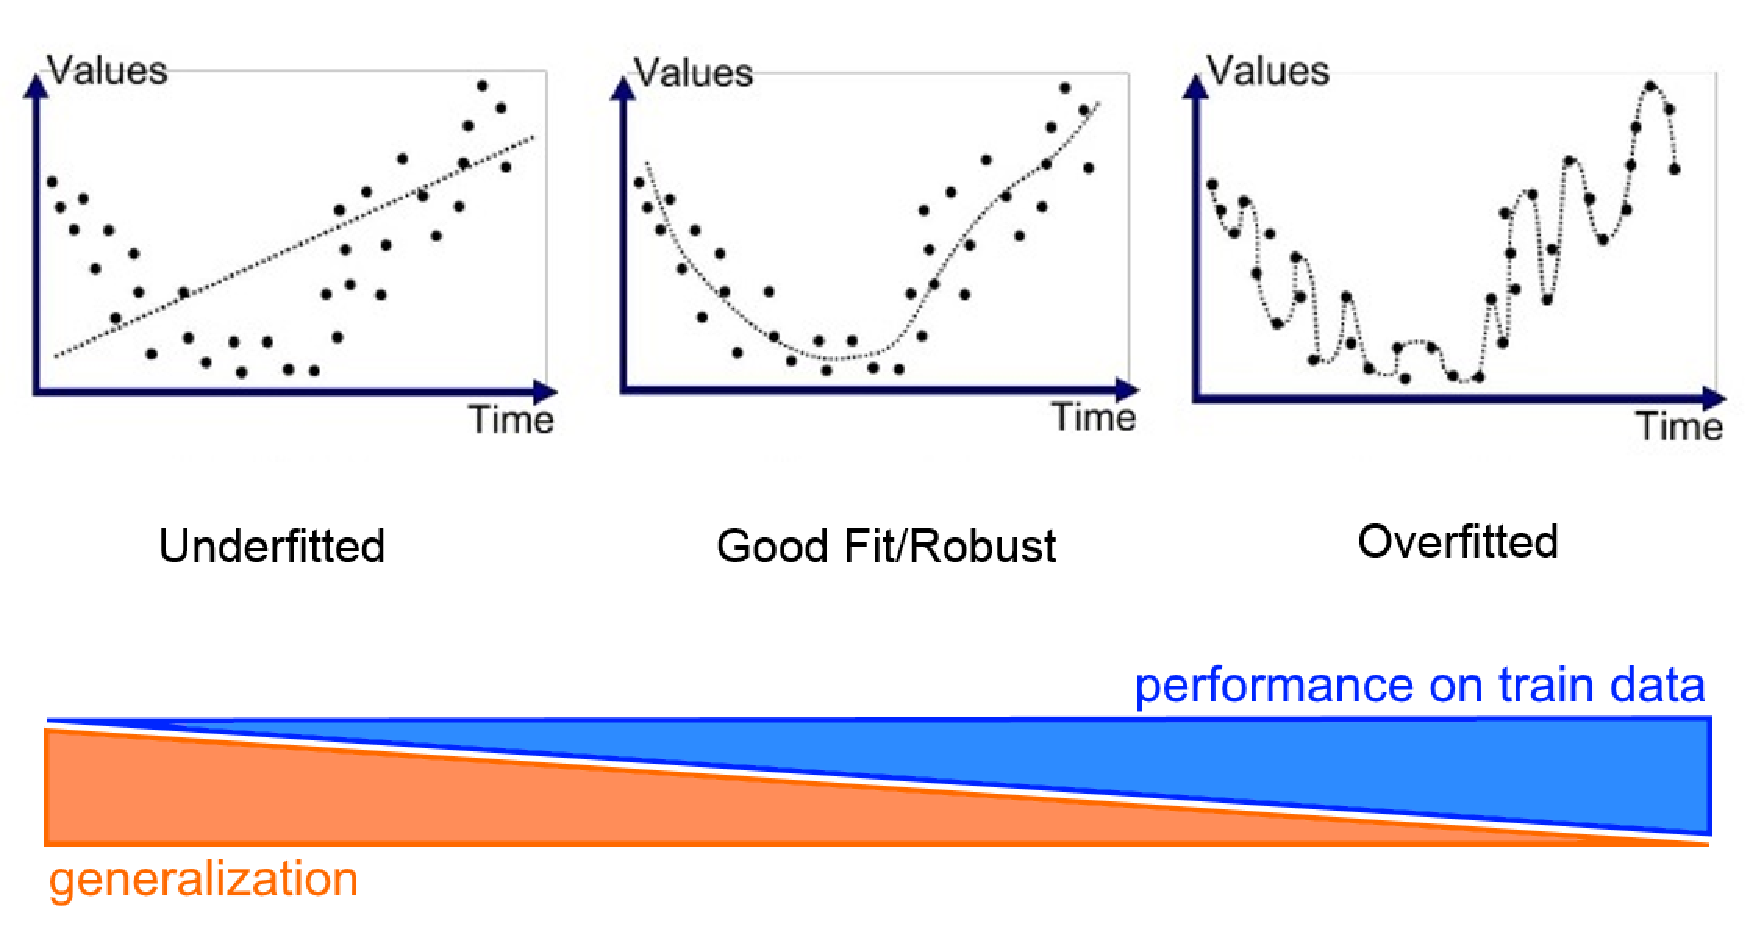
\includegraphics[width=\textwidth]{img/over_underfitting}
   \caption{Visualisation of under- and overfitting on a dataset.}
   \source{altered by the author, https://medium.com/greyatom/what-is-underfitting-and-overfitting-in-machine-learning-and-how-to-deal-with-it-6803a989c76, accessed: 29.03.2019}
   \label{fig:over_underfitting}
\end{figure}

Supervised learning on the other hand happens when the model is fed and trained upon example data with their correct classification labels present. The term 'supervised' therefore relates to the fact that presumably a human told the model which data points belong to which class. This approach is understandably more laborious because the creation of a labelled training's dataset takes time. The benefits are generally better performing models and the possibility to directly test the model. The testing is done by splitting the original training's dataset into two parts. Generally, a bigger portion ($\sim$ 75\%) is used for training the model and the other one ($\sim$ 25\%) - which the model has never seen during the fitting phase - is used to test the model's performance. \\
\newline
Frequently used terms in relation to ML are under- and overfitting. These terms correspond to two extremes of how the model and its incorporated (boundary-) function is fitted to the provided test-data (see points in figure \ref{fig:over_underfitting}). Underfitting describes the state, where the model does not seem to extract and comprehend any logic from the dataset and therefore over-generalises the classification or regression problem at hand (see outer left graph of figure \ref{fig:over_underfitting}). \\
The other extreme is known by the term overfitting where the model tries to correctly classify every single training-data point to its proper class. This results in the model being extremely tuned to the provided training-data but not being able to generalise well on new unseen data (see outer right graph in figure \ref{fig:over_underfitting}). In other words overfitting basically means that the model learned the training's data by hard which results in misleadingly high performance scores. The process of finding the balance between a model that is able to generalise on new data while identifying the underlying data-patterns is further described in section \ref{ml_text_data}.

\section{Ethics}

Drawing upon crowed sourced big-data is inevitably shadowed by ethical controversies. Using GPS locations and other sensitive data to identify and analyse patterns of human behaviour is rightfully criticised and sometimes considered unethical practise.\\
We are only talking about data that is publicly available, data that the user decided to share on the web on his or her own behalf - or is it?. The paper of \parencite{Estima2016} shows that not the entirety of data is voluntarily shared. Did the user sign up for his or her data to be systematically analysed? This depends on the Terms of Service (TOS) of the corresponding SMP which are hardly ever read by the consumer.\\
One has to understand the potential power this data possess. Having access to hundreds of personalised media objects of a specific social media user enables analytics to construct a blueprint of that person. This blueprint can encompasses the persons political orientation, its home and work location, preferences and dislikes as well as daily routines. Personalised advertisement would then be the smallest resulting threat. Interpersonal surveillance \parencite{Trottier2017}, stalking \parencite{Lyndon2011} or potential blackmailing through acquired sensitive information are by far greater and current threats. Additionally, it is unclear from a data-researcher point of view how to deal with encounters of media objects that indicate illegal behaviour e.g littering, assault or theft.\\

With that being said I personally think that the ethical discrepancy is legitimately continuously discussed in this context. Showing how the data and the anonymity of the authors is treated as well as the goal a project pursues are key elements that determine in my opinion if ethical terms are violated or not. 







\cleardoublepage
\chapter{Materials and methods} \label{material_methods}

\section{Research area} \label{research_area}
The Canton of Zug was chosen by the author - who was raised in Cham - as the area of interest since important local knowledge was already present. The specific areas for which social media data (SMD) was acquired are visible in the map below (see figure \ref{fig:research_area}). The turquoise area resembles the political border of the Canton of Zug for which SMD for the social media platforms (SMP) Flickr and Foursquare were collected. The purple area is included in the above mentioned perimeter of the Canton of Zug and consists of three major areas. In the North lies the \lq Lorzenebene\rq (plane of the river Lorze). This area is of special interest to the cantonal authorities due to its local recreation value. An overall concept - named \lq Leitbild Lorzenebene\rq has been created for it which was used as reference in this thesis \cite{BaudirektiondesKantonsZug2012LeitbildBericht}. The second area resembles the jurisdiction of the City of Zug which partly encompasses the \lq Lorzenebene\rq . This area is distinctive by its internal urban gradient which increases towards the city centre as well as the long reaching lake side. The last area furthest South consists of the three mountains \lq Zuger-, Walchwiler-, Rossberg\rq which are likewise part of an development concept \cite{Berchtold2011EntwicklungsleitbildRossberg} of the Canton of Zug due to their sport and recreation value. \\
There is no perimeter concordance due to varying constraints in the data acquisition between the different social media platforms which will be illustrated further down in section \ref{data_acquisition}.

\begin{figure}[h]
   \centering
   \includegraphics[width=0.75\textwidth]{img/overview_research_area_w_Lorzenebene.eps}
   \caption{Overview over the data acquisition perimeters}
   \label{fig:research_area}
\end{figure}


\section{Data acquisition and composition} \label{data_acquisition}
The following subsections will elaborate on the data-acquisition process and the data-composition of the three SMP used in this thesis. 

\subsection{Instagram} \label{instagram}
Instagram is a SMP which supports the sharing of geo-referenced image and video content. The platform is mostly financed by web-advertisement and belongs to \textit{Facebook Inc.} It can be accessed via the URL \texttt{https://www.instagram.com/} or the corresponding mobile application.
Instagram held roughly 2\rq529\rq000 users in Switzerland on January 2019 which accounted for 29.4\% of its population. People aged 25 to 34 were the largest user group (780\rq 000). The gender distribution was at 49.4\% women and 50.6\% men \cite{NapoleonCat2019NoTitle}. This popularity was the determining factor that lead to including Instagram data into this thesis.\\

\subsubsection{Query} \label{netlytic}
Licensed Instagram data of the research area visible in figure \ref{fig:research_area} has been collected via the cloud-based text and social media analyser \textit{Netlytic}. \textit{Netlytic} can be accessed via \texttt{https://netlytic.org/} and allows for hashtag (\# + keyword) or location driven queries. Former allows to search for Instagram media objects by providing decisive keywords which are preceded by a \lq \#\rq. The latter was used in the scope of this thesis which allows location based query for Instagram media objects of public accounts in a 5km radius around a given point. The used \textit{Netlytic} query points with their given perimeter are visible in figure \ref{fig:research_area}. The exact latitude / longitude coordinate pairs are the following:\\
\begin{enumerate}
  \item 47.177068, 8.494803
  \item 47.129913, 8.533604
  \item 47.104457, 8.570291
\end{enumerate}

\subsubsection{Time-span} \label{Instagram_timespan}
Data collection has been continuously performed over all three queries from the 30.09.2018 till the 11.12.2018. Due to the retirement of the Instagram Application Program Interface (API) on the 11.12.2018 \cite{Instagram2018InstagramRetirement} this period could not be extended.

\subsubsection{Data} \label{Instagram_data}
The data-collection accounted for 28\rq246 raw Instagram media objects. After the dominant authors and bulk-upload data-processing steps referenced further down (see chapter (\ref{data_processing}) 11\rq777 remained.
The data provided by \textit{Netlytic} came in the Comma Separated Values (CSV) format. Every media object was provided with the following information entities with the appropriate PostgreSQL data type in square brackets:
\begin{itemize}
    \item id : Unique media object identifier. [varchar(30)] if the media object contains location information, [numeric(20)] if not.
    \item latitude and longitude : Coordinate information in the WGS84 reference system of a specific Instagram location [double precision]
    \item link : URL to the actual media object on \texttt{https://www.Instagram.com/} [text]
    \item media-link : URL directing solely to the image content [text]
    \item publication date : Date and time when the media object was uploaded with the data-format YYYY-MM-DD HH:MM:SS [timestamp]
    \item author : The Instagram username of the media object author [text]
    \item title : User generated media object title [text]
    \item description : User generated media object description [text] 
    \item like-count : Amount of likes the media object received on the SMP Instagram
\end{itemize}

\paragraph{Location tag}
The provided location information or tag consists of the above mentioned coordinates of a Instagram location. Instagram locations are points of interest which can be user-generated and do not represent the actual precise coordinates where the media object was created. This has been implemented by Facebook as a further step to preserve the Instagram users anonymity by mitigating the divulging of sensitive location data. This implies that media objects that do not originate from the same location can still be \lq snapped\rq to the same Instagram location and therefore show the same coordinate pair in the meta-data \cite{InstagramTags}.
It has been shown that roughly 85\% of Instagram media objects lack a location tag \cite{2018InstagramTags} and most users only use them on vacation or when being abroad.
Additional location related information (address) was gathered for all the media objects via the official Instagram API. More information can be found in chapter \ref{sec: XXXXX}


\subsection{Flickr} \label{flickr}
Flickr is photo sharing website (\texttt{https://www.flickr.com/}) that allows users to upload geo-reverenced images similar to Instagram. The corresponding free of charge Flickr API gives access to the entire database of Flickr media objects since the launch of the platform in the year 2005. The popularity of Flickr according to the\lq Alexa Global Rank\rq lies at 349 \cite{Alexa.com2019AlexaFlickr} which is significantly lower than to the one of Instagram which lies at 16 \cite{Alexa.com2019AlexaInstagram}. Flickr still plays an important role also as data foundation for scientific studies due to the simple and unbounded data-access. <ADD REFERENCES>
DEMOGRPAHIC INFORMATION
WHY WAS IT CHOSEN
\subsubsection{Query} \label{flickr_query}
The entire Flickr database was queried via the publicly accessible official Flickr API. Media objects with a geo-reference-accuracy level of 12 or higher (maximum of 16) were of interest which resolves to city level up to street level. Queries were conducted by inputting several different bounding boxes which together cover the entire perimeter of the legal boundaries of the canton of Zug. Each bounding box was defined by two coordinate pairs, describing the bottom left and top right corner of a rectangle. This process of subdividing the area was necessary due to a maximum return threshold of 4\rq000 media objects per request. Therefore, to ensure the acquisition of the entire available data-set each bounding box had to hold less than 4\rq000 media objects.
\subsubsection{Time-span} \label{flickr_timespan}
The all the individual bounding-box API requests described above were queried for the time-spawn 2005 (launch of the SMP Flickr) until the 23rd of November 2018. 
\subsubsection{Data} \label{flickr_data}
The data that was returned by the Flickr API was in the JavaScript Object Notation (JSON) format. The following information has been extracted for every Flickr media object with the appropriate PostgreSQL data types in square brackets:\\

\begin{itemize}
    \item id : Unique media object identifier [bigint]
    \item latitude and longitude : Coordinate information in the WGS84 reference system [double precision]
    \item link : URL to the actual media object in the format \texttt{https://www.flickr.com/photos/[author]/[ID]/} [text]
    \item date taken : Time-stamp from the image meta-data stating when it was taken. 
    \item publication date : Time-stamp when the media object was uploaded to Flickr with the data-format MM/DD/YYYY HH:MM:SS [time-stamp]
    \item author : The Flickr username of the media object author [text]
    \item author id : Unique author identifier [text] 
    \item author origin : User given geographical information regarding the authors origin [text]
    \item title : User generated media object title [text]
    \item description : User generated media object description [text]
    \item tags : Keywords similar to Instagram hashtags that describe the media object [text]
    \item views : Amount of media object calls [bigint]
    \item favorites : Amount of approves - similar to \lq likes\rq on Instagram - a media object received by other Flickr users [bigint]
\end{itemize}

\paragraph{Location tag}
Unlike Instagram provides Flickr location information or tags that represent the actual geographical position where the provided image was taken. This geotag is extracted from the meta-data of the image itself and can come in different accuracies ranging from 0 (global scale) to 16 (street level) dependant on the users preference or the GPS signal strength. \\
Additional location related information (address and location type) was gathered for all the media objects via the Google Geocoding API. More information can be found in chapter \ref{sec: XXXXX}

\subsection{Foursquare} \label{foursquare}
Foursquare is a platform which enables users to rate and share their visits and experiences to certain establishments (referred to as venues). All the stored \lq infrastructure\rq which is categorised into different sectors such as \lq Travel & Transport\rq, \lq Arts and Entertainment\rq but also \lq Outdoors & Recreation\rq can be accessed via the official Foursquare API.
DEMOGRAPHIC INFORMATION
WHY WAS IT CHOSEN
\subsubsection{Query} \label{foursquare_query}
The following two API endpoints which return different information were used for this thesis.
\paragraph{Venue search (regular endpoint)} \label{foursquare_endpoint1}
The first step of the information acquirement involved a spatial search for venue ids of the category \lq Outdoors & Recreation\rq that lie within the research area boundaries. This request was done with the regular venue search API endpoint. There was a limitation to the maximum number of results per request, similar to the bounding box request of Flickr. Therefore, a similar spatial subdivision of the research areas was used to query all the available venues, so that each individual request returned less than 50 results.
\paragraph{Acquiring venue details (premium endpoint)} \label{foursquare_endpoint2}
To obtain more specific information about each venue, a second (premium) Foursquare API endpoint was used. This venue details endpoint only allowed 50 requests per day for regular users which spread the data acquisition over 9 days. Insight among others on a more concrete subcategory description, the formatted address, the user rating as well as if the venue was verified or not was the result.

\subsubsection{Data} \label{fq_data}
The data returned by the Foursqure API and the above mentioned endpoints was in the JSON format - the same as the Flickr data.
Only the following excerpt of the returned venue meta-data was used with the appropriate PostgreSQL data types in square brackets: \\
\begin{itemize}
    \item venue id : Unique venue identifier [text]
    \item venue name : Locally used name to address the venue [text]
    \item latitude and longitude : Coordinate information in the WGS84 reference system [double precision]
    \item country name : Name of the country the venue is located in - used as additional data-verification [text]
    \item rating : Venue rating generated through Foursquare users [real]
    \item category id : Unique Foursquare venue category identifier [text]
    \item category name : Foursquare venue category name
    \item verified : Takes the values TRUE or FALSE. States if the venue data is verified by Foursquare
\end{itemize}

Additional location related information (address and location type) was gathered for all the media objects via the Google Geocoding API. More information can be found in chapter \ref{sec: XXXXX}

\subsubsection{Data verification} \label{foursquare_data_verification}
The data verification on Foursquare is not an automated process. It is done by manual supervision of Foursquare personnel. If a business can claim their venue which will initiate the Foursquare verification process. This processing is linked to a fee of roughly 20 USD for venues outside of the United States of America \cite{Foursquare2019FoursquareClaim}. \\
Of all 405 venues located inside the canton of Zug, 13 (3.2\%) are verified according to the data provided by the foursquare API. The remaining non-verified venues of the categories: scenic outlook, playground, athletics & sport, farm, (nudist) beach, lake, trail, golf course, mountain, campground, bathing area, outdoors & recreation, harbour, recreation centre, dog run, forest, pedestrian plaza, waterfront, basketball court, river, bike trail and skate park were evaluated by the author - who grew up in the area - to its best knowledge. XY venues belonged to said categories of which XY were verified by the author of this thesis.

\section{Database Setup} \label{database_setup}
During the course of this thesis a PostgreSQL database (\texttt{https://www.postgresql.org/}) was used which functioned as a centralised place to store the Flickr, Instagram and Foursquare data related to this project. The advantage of this approach compared to reading and storing in common txt- or csv-files is the possibility of computational efficient data-retrieval as by indexing conditional columns and data-manipulation through SQL queries. SQL is a standalone language for relational database management systems (RDBMS) which allows among other, smart table joins through primary and foreign key relation and conditional statements for advanced filtering \cite{PostgreSQL2019PostgreSQLDocumentation}.\\
Additionally, a Graphical User Interface (GUI) named pgAdmin4 (\texttt{https://www.pgadmin.org/}) - which is compatible with PostgreSQL - was used for the manually performed training-data verification process that is described in chapter \ref{XY}.\\
The following tables were created for the housing of the used data in this format: [object-type]\_[data-origin]\_[data-source] \\
\newline

Media object tables:\\
\begin{itemize}
    \item media\_objects\_cantonzug\_flickr
    \item media\_objects\_unionzug\_instagram
    \item media\_objects\_trainingdata\_instagram
    \item media\_objects\_cantonzug\_foursquare
\end{itemize}
\newline
Location tables:\\
\begin{itemize}
    \item locations\_cantonzug\_flickr
    \item locations\_unionzug\_instagram
\end{itemize}

In more detail, the media object tables store all data related to an object retrieved from one of the three SMP as stated in the corresponding subchapters above. Furthermore are the outputs from the data- and text-processing steps (see chapter \ref{XY}) stored in the database.\\ 
The Instagram and Flickr media object tables are linked via a primary key to the corresponding locations table, where unique media object location information is separately stored to reduce redundancy. This information exceeds the basic coordinates provided by the Flickr API and the stand-alone user generated location provided by Netlytic (Instagram) by acquiring additional geographic information via Googles Geocoding API and the Instagram API respectively (see chapter \ref{XXXX}). Time-stamps were normalised across all SMP to the YYYY-MM-DD HH-MM-SS format \\
\newline
The exact structure and table specific content of the database is visible in figure \ref{fig:database}

\begin{figure}[h]
   \centering
   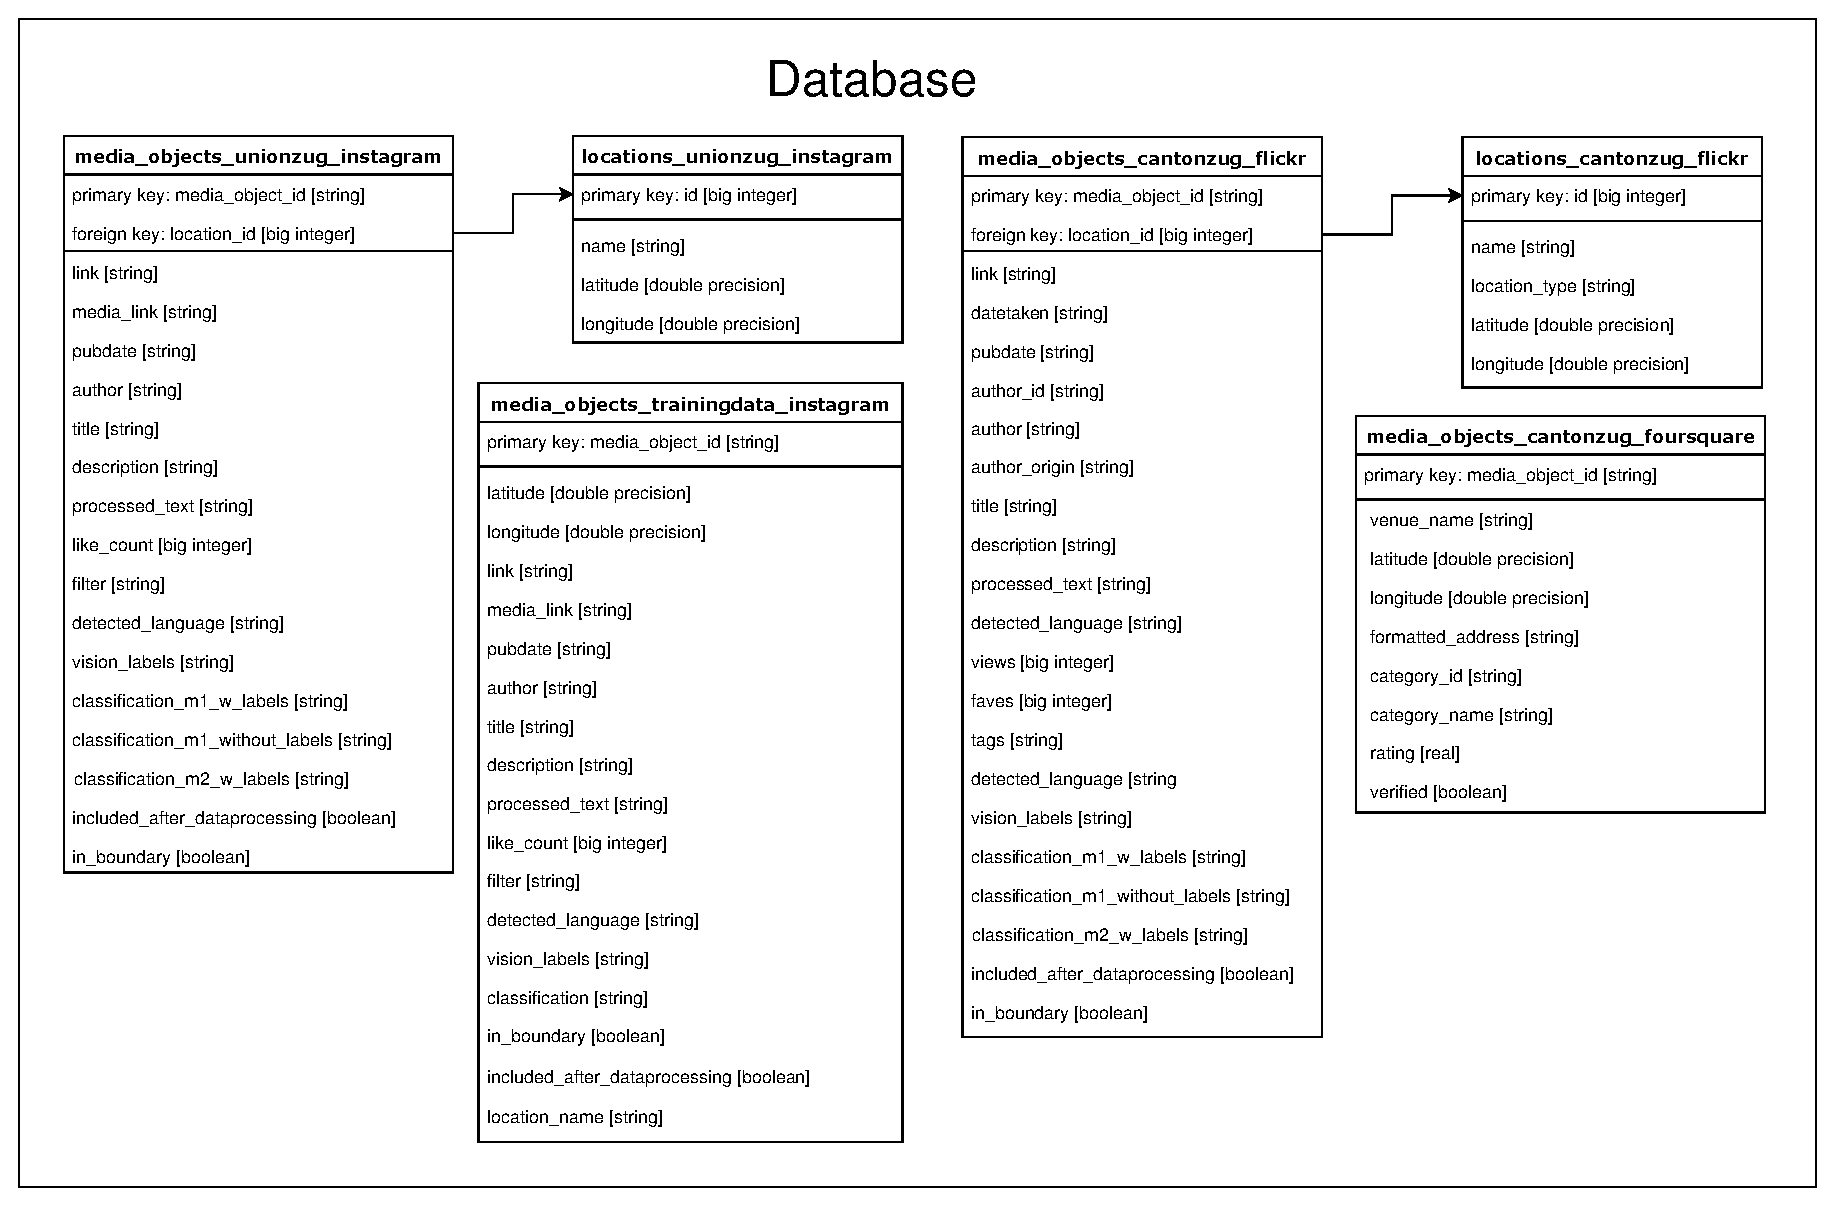
\includegraphics[width=0.75\textwidth]{img/fusion_db_overview.eps}
   \caption{Visualisation of the database, its associated tables and columns}
   \label{fig:database}
\end{figure}

\section{Data-processing} \label{data_processing}
The following processes cover the entire workflow of data manipulation on the database in the order they were executed.
\subsection{Merging of Instagram files} \label{netlytic_files_merge}
In total, three different, partly spatially overlapping Instagram queries were run via Netlytic. All of them returned one CSV file. they were merged to reduce the complexity of handling multiple files for the consecutive processes. Media object duplicates were also addressed in this step. This entire data-processing step was not needed for the Flickr-data since merging and duplicates were already handled during the data-mining.

\subsection{Acquisition of additional location information} \label{add_location_data}
Auxiliary, more detailed location information regarding the spatial origin of the media objects in the database were acquired. The following two subchapters will elaborate on this process for the different data sources Instagram and Flickr.

\subsubsection{Via the Instagram API}
The Instagram data that was provided by Netlytic was enhanced by using the \texttt{GET/locations/location-id} endpoint of the official Instagram API. Newly acquired information encompassed the Instagram location-name.

\subsubsection{Via the Google Geocoding API}
Each coordinate of every Flickr media object was run through the Google Geocoding API. Detailed information regarding the media objects address and location type was returned. The location type attribute is evidence of the API\rq s accuracy. Everything besides 'ROOFTOP' returns an address that is close but not exactly at the given coordinate and therefore an approximation.\\
The API has been called by modifiying the following HTTPS-request:\\
\texttt{https://maps.googleapis.com/maps/api/geocode/json?latlng=[latitude,longitude]&key=[API_KEY]}

\subsection{Populating the database} \label{populate_db}
The merged Instagram CSV-files and the Flickr CSV-files which were extended by the addititional location information descirbed in the subchapters above were used to populate the inital PostgeSQL database. This process was entirely done through the Python script provided in the Appendix \ref{XY} and the needed \textit{psycopg 2} library that functioned as linkage.

\subsection{Check the \lq in boundary\rq condition} \label{in_boundary}
Due to the data querying span which does not entirely match the actual research area perimeters, each acquired media object had to be checked to be inside the given perimeter boundary. This process was done manually with the open source Geographical Information Software (GIS) QGIS. The point data of all media objects is clipped to the given research area. All remaining points / media objects are than exported to a new file and read by the script which automatically updates the \lq in\_boundary\rq column in the corresponding database table to TRUE.








%\chapter{Working with \LaTeX\ }\label{sec:working}
This chapter explains how to typeset some of the most common elements contained in a technical report using \LaTeX.

\section{Headings}
Your report can be structured using several different types of headings. Use the commands \texttt{\textbackslash chapter\{.\}}, \texttt{\textbackslash section\{.\}}, \texttt{\textbackslash subsection\{.\}}, and \texttt{\textbackslash subsubsection\{.\}}. Use the asterisk symbol \texttt{*} to suppress numbering of a certain heading if necessary, for example, \texttt{\textbackslash section*\{.\}}.

\section{References and Footnotes}\label{sec:references}
References to literature are included using the command \texttt{\textbackslash
cite\{.\}}. For example \cite{optreg,motsys}. Your references must be entered in the file \texttt{bibliography.bib}. Making changes or adding new references in the bibliography file can be done manually or by using specialized software such as \textit{JabRef} which is free of charge.
 
Cross-referencing within the text is easily done using \texttt{\textbackslash label\{.\}} and \texttt{\textbackslash ref\{.\}}. For example, this paragraph is part of chapter~\ref{sec:working}; more specifically section~\ref{sec:references} on page~\pageref{sec:references}. You will need to compile your document twice in order for the cross-referencing to be updated.

Footnotes\footnote{The use of footnotes is generally not recommended.} are added using the command \texttt{\textbackslash footnote\{.\}}, but try to avoid the used of footnotes altogether.

\section{Lists}\label{sec:lists}
Three types of list-environments are commonly used: \texttt{itemize}, \texttt{enumerate}, and \texttt{description}. The following example uses \texttt{itemize} to create a list without numbering
\begin{itemize}
  \item point one; and
  \item point two
\end{itemize}
created using
\begin{verbatim}
\begin{itemize}
  \item point one; and
  \item point two
\end{itemize}
\end{verbatim}

The following example uses \texttt{enumerate} to create a list with numbering
\begin{enumerate}
  \item point one; and
  \item point two
\end{enumerate}
created using
\begin{verbatim}
\begin{enumerate}
  \item point one; and
  \item point two
\end{enumerate}
\end{verbatim}

The following example uses \texttt{description} to create a list with custom text as bullet-points
\begin{description}
  \item[P1] point one; and
  \item[P2] point two
\end{description}
created using
\begin{verbatim}
\begin{description}
  \item[P1] point one; and
  \item[P2] point two
\end{description}
\end{verbatim}


\section{Tables}\label{sec:tables}
Table~\ref{tab:table} shows an example of a simple table-layout. Try to avoid vertical lines on tables. The Internet contains countless resources on how to create special elements and structures in tables such as cells spanning multiple rows, rotated text, sideways tables, justification of cell elements, etc.
\begin{table}[ht]
\begin{center}
\caption{Driving cycle data of ECE-15, EUDC, and NEDC.}\vspace{1ex}
\label{tab:table}
\begin{tabular}{llccc}\hline
Description & Unit & ECE & EUDC & NEDC \\ \hline
Duration & s & 780 & 400 & 1180 \\
Distance & km & 4.052 & 6.955 & 11.007 \\
Average velocity & km/h & 18.7 &  62.6 & 33.6 \\
Idle speed & \% & 36 & 10 & 27 \\ \hline
\end{tabular}
\end{center}
\end{table}

This table was created using
\begin{verbatim}
\begin{table}[ht]
\begin{center}
\caption{Driving cycle data of ECE-15, EUDC, and NEDC.}\vspace{1ex}
\label{tab:table}
\begin{tabular}{llccc}\hline
Description & Unit & ECE & EUDC & NEDC \\ \hline
Duration & s & 780 & 400 & 1180 \\
Distance & km & 4.052 & 6.955 & 11.007 \\
Average velocity & km/h & 18.7 &  62.6 & 33.6 \\
Idle speed & \% & 36 & 10 & 27 \\ \hline
\end{tabular}
\end{center}
\end{table}
\end{verbatim}
Table~\ref{tab:table_advanced} shows a more advanced version of Tab.~\ref{tab:table} using the \texttt{booktabs} package. Inspect the source code of this document to see how this was done.
\begin{table}[ht]
\begin{center}
\small
\caption{Driving cycle data of ECE-15, EUDC, and NEDC.}\vspace{1ex}
\label{tab:table_advanced}
\begin{tabular}{@{}lcccc@{}}\toprule[1.5pt]
& & \multicolumn{3}{c}{\bf Driving cycle}\\
\cmidrule{3-5}
Description & Unit & {ECE} & {EUDC} & {NEDC} \\ \midrule
Duration & \unit[]{s} & 780 & 400 & 1180 \\
Distance & \unit[]{km} & 4.052 & 6.955 & 11.007 \\
Average velocity & \unitfrac[]{km}{h} & 18.7 &  62.6 & 33.6 \\
Idle speed & \unit[]{\%} & 36 & 10 & 27 \\ \bottomrule[1.5pt]
\end{tabular}
\end{center}
\end{table}



\section{Working with Units}
The package \texttt{\textbackslash usepackage\{units\}} enables two useful commands, namely \texttt{\textbackslash unit[.]\{.\}} and \\ \texttt{\textbackslash unitfrac[.]\{.\}\{.\}}. Use these commands to display units in a concise way, for example
\begin{align}
\delta t &= \unit[1]{s}\\
v &= \unitfrac[5]{m}{s}.
\end{align}
This example was done using
\begin{verbatim}
\begin{align}
\delta t &= \unit[1]{s}\\
v &= \unitfrac[5]{m}{s}.
\end{align}
\end{verbatim}

\section{Including Graphics}\label{sec:epsgraph}
It is recommended that you only use encapsulated post-script graphics \texttt{.eps} in your report. If you mix \texttt{.eps} with other formats such as \texttt{.png}, \texttt{.jpeg} or \texttt{.gif}, you will most likely not be able to compile your report without errors. Note that figures created in \textsc{Matlab} are easily saved in \texttt{.eps} format.

The inclusion of a figure can be done in the following way:
\begin{verbatim}
\begin{figure}[ht]
   \centering
   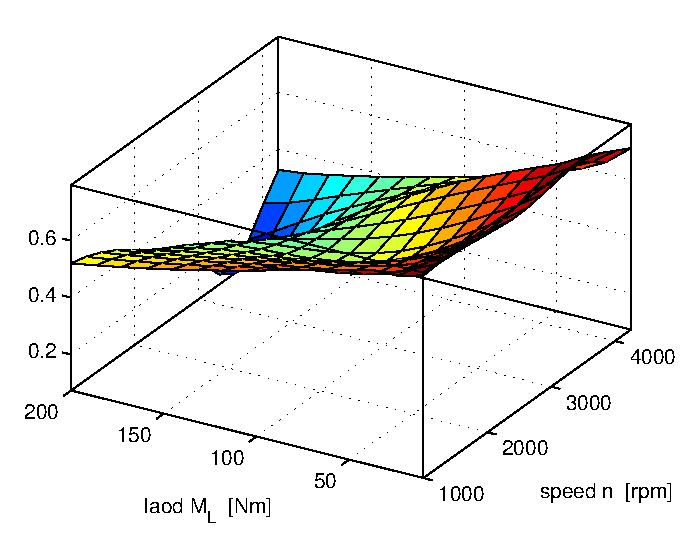
\includegraphics[width=0.75\textwidth]{img/k_surf.eps}
   \caption{Example of a figure.}
   \label{img:k_surf}
\end{figure}
\end{verbatim}

\begin{figure}[ht]
   \centering
   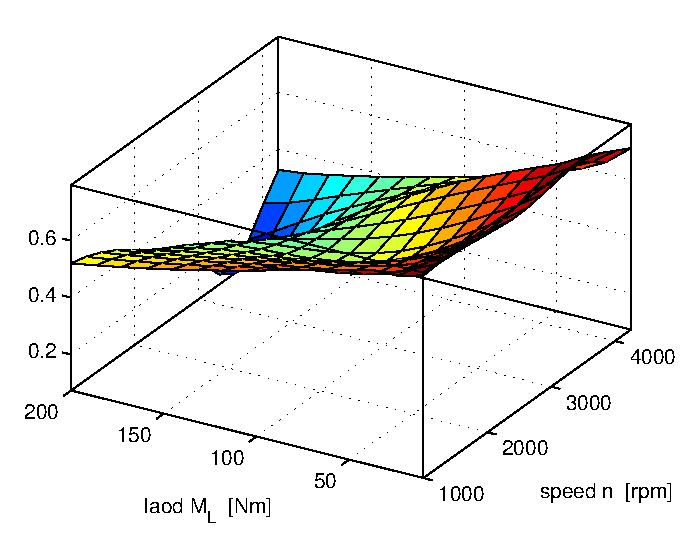
\includegraphics[width=0.75\textwidth]{img/k_surf.eps}
   \caption{Example of a figure.}
   \label{img:k_surf}
\end{figure}

Two figures are displayed next to each other using
\begin{verbatim}
\begin{figure}[ht]
  \begin{minipage}[t]{0.48\textwidth}
    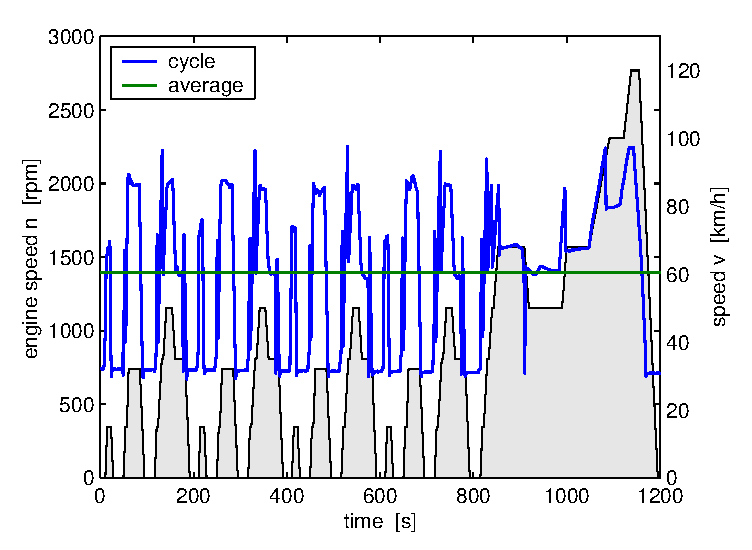
\includegraphics[width = \textwidth]{img/cycle_we.eps}
  \end{minipage}
  \hfill
  \begin{minipage}[t]{0.48\textwidth}
    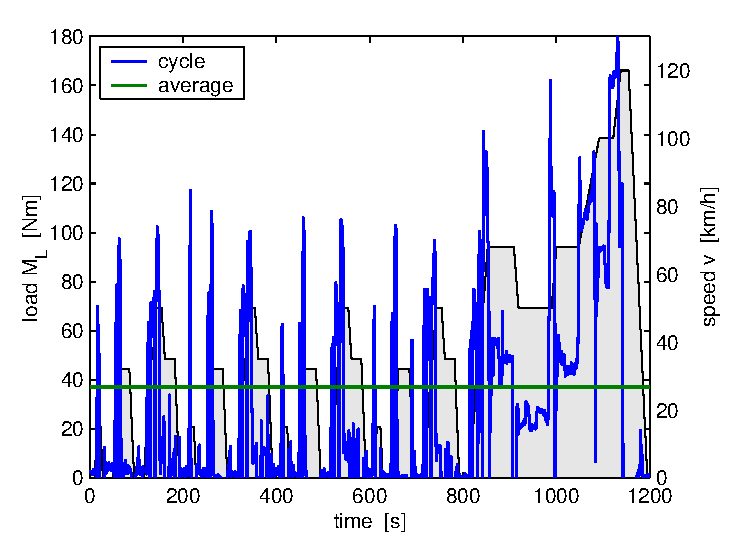
\includegraphics[width = \textwidth]{img/cycle_ml.eps}
  \end{minipage}
  \caption{Two figures next to each other.}
  \label{img:cycle}
\end{figure}
\end{verbatim}

\begin{figure}[ht]
  \begin{minipage}[t]{0.48\textwidth}
    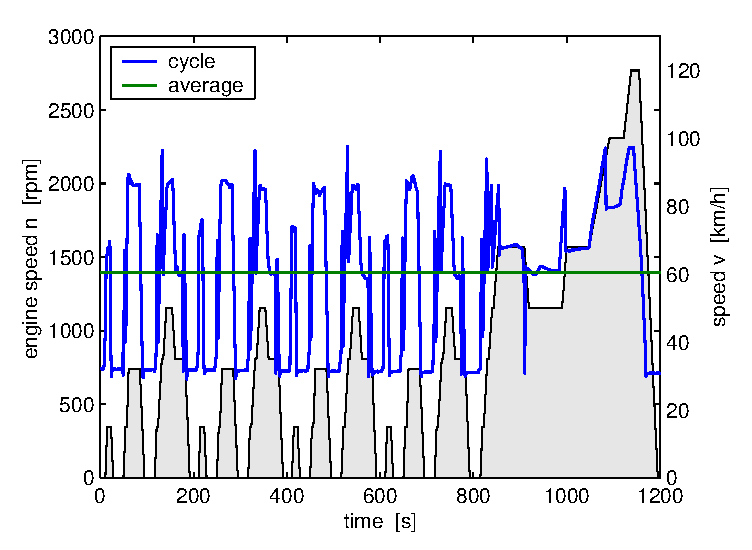
\includegraphics[width = \textwidth]{img/cycle_we.eps}
  \end{minipage}
  \hfill
  \begin{minipage}[t]{0.48\textwidth}
    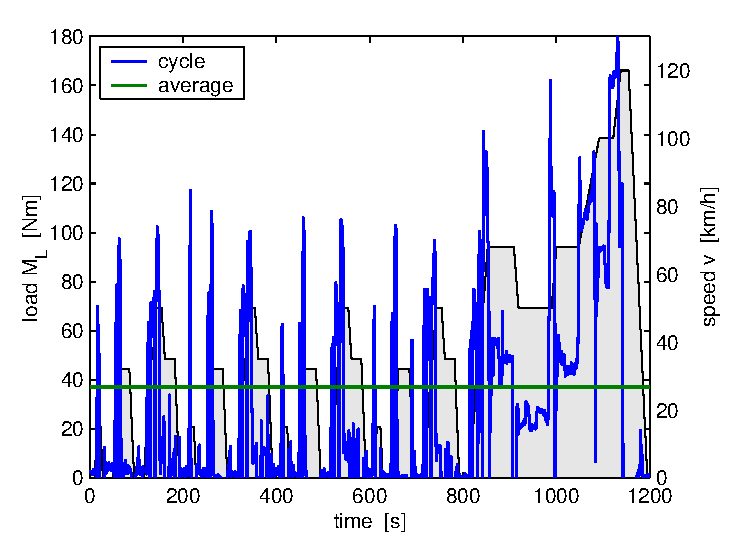
\includegraphics[width = \textwidth]{img/cycle_ml.eps}
  \end{minipage}
  \caption{Two figures next to each other.}
  \label{img:cycle}
\end{figure}

The positioning parameter \texttt{h} (here) forces your figure to be placed in the current position relative to your text. You may add \texttt{t} (top), \texttt{b} (bottom), and/or \texttt{p} (page) to allow for more flexible positioning within your document. For instance, \texttt{[tb]} forces your figure to be placed either on the top or bottom of a page.


\section{Equations}\label{sec:math}
The most common way to include equations is using the \texttt{equation} environment.
\begin{equation}\label{eq:p_me0f}
 p_\mathrm{me0f}(T_e,\omega_e) \ = \ k_1(T_e) \cdot (k_2+k_3 S^2
 \omega_e^2) \cdot \Pi_\mathrm{max} \cdot \sqrt{\frac{k_4}{B}} \, .
\end{equation}
It is recommended to use \texttt{\textbackslash mathrm\{.\}} for subscripts comprising more than two letters since it reduces the width of the subscript significantly and improves readability. The corresponding code is
\begin{verbatim}
\begin{equation}\label{eq:p_me0f}
 p_\mathrm{me0f}(T_e,\omega_e) \ = \ k_1(T_e) \cdot (k_2+k_3 S^2
 \omega_e^2) \cdot \Pi_\mathrm{max} \cdot \sqrt{\frac{k_4}{B}} \, .
\end{equation}
\end{verbatim}
Equations, such as Eq.~\eqref{eq:p_me0f}, may be referenced using \texttt{\textbackslash eqref\{.\}}. In-line mathematical content is created using \texttt{\$.\$}, for example $a^2+b^2=c^2$. It is practically possible to typeset any equation in \LaTeX. Equation~\eqref{eq:advanced} shows an example of a more advance structure.
\begin{equation}\label{eq:advanced}
x^k_n(i) = \left\{\begin{array}{ll}y(i) & \text{if}\quad x^k_{n-1}(i)\leq \mathbf{x}\\
z(i) & \text{otherwise}\end{array}\right., \text{for}\quad i=\{1,\ldots,N\}.
\end{equation}



\section{Including Code in your Document}
Include samples from your Matlab code using the \texttt{lstlistings} environment, for example
\lstset{language=Matlab,numbers=none}
\begin{lstlisting}[frame=lines]
% Evaluate y = 2x
for i = 1:length(x)

  y(i) = 2*x(i);

end
\end{lstlisting}
This example was created using
\begin{verbatim}
\lstset{language=Matlab,numbers=none}
\begin{lstlisting}[frame=lines]
% Evaluate y = 2x
for i = 1:length(x)

  y(i) = 2*x(i);

end
\end{lstlisting}
\end{verbatim}
where \texttt{\textbackslash usepackage\{mcode\}} must be included in the preamble of your document. If you want to include the entire content of a file \texttt{mycode.m} in your document, simply input the path to \texttt{mycode.m} instead of pasting the entire content into your \TeX -file
\begin{verbatim}
\lstset{language=Matlab,numbers=left}
\lstinputlisting{path/to/mycode.m}
\end{verbatim}
Including the path to your m-file also ensures that the code in your report is always up-to-date. The \texttt{\textbackslash lstset\{language=Matlab\}} command ensures that \textsc{Matlab} syntax definitions are used, but many other languages are recognised as well such as \texttt{Fortran} and \texttt{C++}.

\cleardoublepage
\chapter{Results} \label{results}
This chapter will encompass the result of the two ML models for NBRA prediction in Instagram and Flickr media objects as well as the evaluation of the ground truth data consisting of interviews and the passive observation statistic of NBRAs.
\section{Data-processing} \label{results_dataprocessing}
Table \ref{tab:data_reduction_values} provides an overview of the data-reduction for each used dataset as a result of the data-processing described in section \ref{data_processing} which consisted of:
\begin{itemize}
  \item in boundary check
  \item dominant authors exclusion
  \item bulk uploads
\end{itemize}

\begin{table}[h!]
\begin{center}
\caption{Listing of the applied thresholds and the resulting data-reduction of each dataset.}\vspace{1ex}
\label{tab:data_reduction_values}
\begin{tabular}{ccccc}\hline
dataset & excluded top authors & bulk threshold & input & output & data-reduction\\ \hline
Instagram Zug & 6 & 6 & 28'246 & 11'777 & 58.3\% \\
Instagram Zurich Uetliberg & 10 & 5 & 74'742 & 68'522 & 8.3\% \\
Instagram Zurich Dolder & 7 & 5 &  206'454 &  191'584 & 7.2\% \\
Flickr Zug & 12 & 7 &  14'236 &  3'790 & 73.4\% \\ 
Foursquare Zug & - & - & 405 & 378 & 6.7\% \\ \hline
\end{tabular}
\end{center}
\end{table}

The noticeably high data-reduction of the Flickr dataset was mostly due to large total upload numbers of a small share of users. Visible in figure \ref{img:dominant_users_flickr} are Flickr-users (authors) uploading up to 1'190 media objects since the launch of Flickr in the year 2004. As a result roughly 5'700 media objects were removed alone in the 'dominant user' data-processing step.

\begin{figure}[h!]
   \centering
   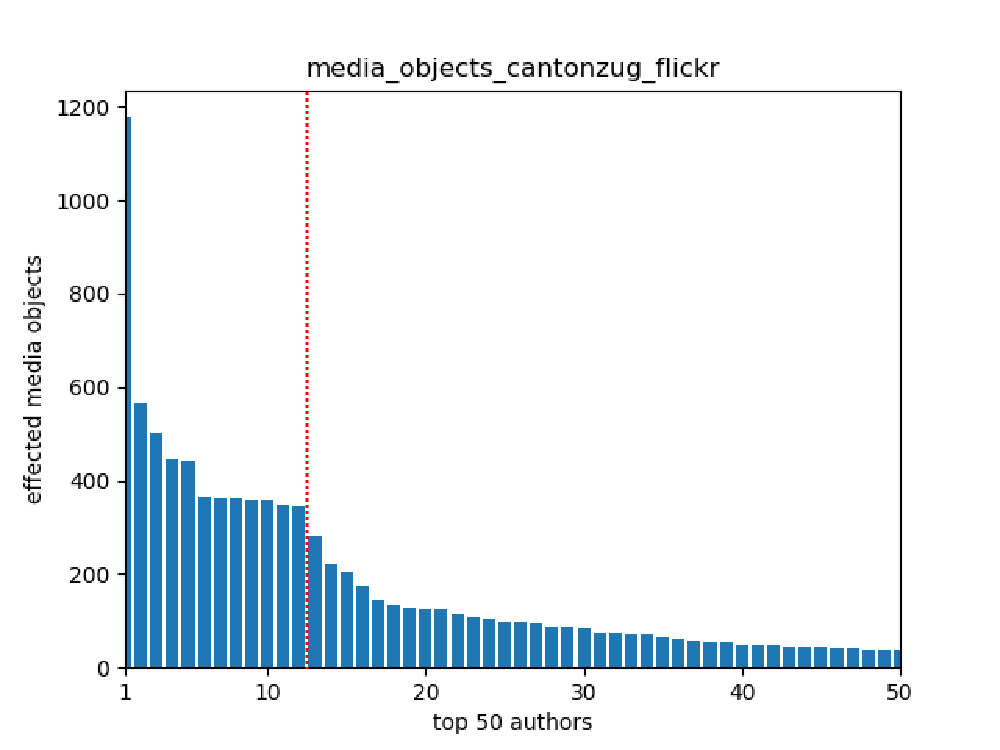
\includegraphics[width=0.75\textwidth]{img/cantonzug_flickr_top50_w_line}
   \caption{Overview of the uploaded media objects of the top 50 Flickr users since 2004 in the Canton of Zug. The top 12 users which account for roughly 5'700 media objects (left to the red line) were excluded from further data-analysis during the 'dominant' user data-processing step.}
   \label{img:dominant_users_flickr}
\end{figure}

As seen in figure \ref{img:bulk_uploads_flickr} an additional, roughly 3'000 Flickr media objects were removed in the 'bulk-upload' process. The y-values of that figure correspond to the potentially removed amount of media objects if a certain threshold on the x-axis is applied. The data visible in this graph only includes media objects which were not already excluded by preceding data-processing steps.

\begin{figure}[h!]
   \centering
   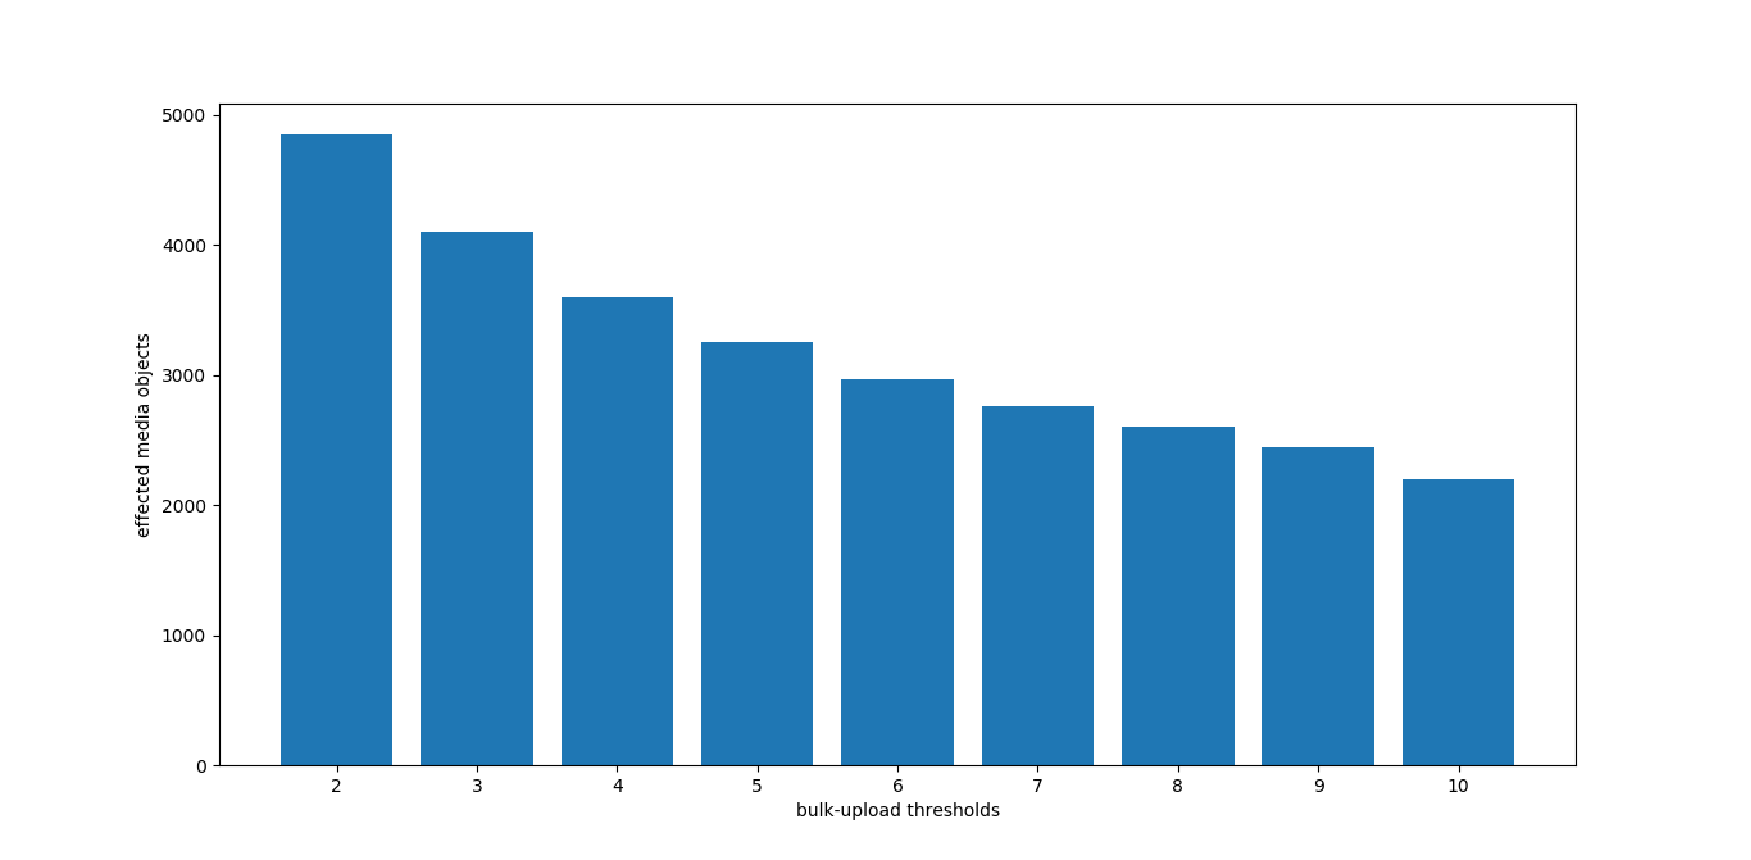
\includegraphics[width=0.75\textwidth]{img/cantonzug_flickr_bulkuploads_cropped.pdf}
   \caption{Shows the impact of different 'bulk-upload' thresholds on the Flickr dataset of the Canton of Zug}
   \label{img:bulk_uploads_flickr}
\end{figure}

Similar graphs to figure \ref{img:dominant_users_flickr} and \ref{img:bulk_uploads_flickr} were created for all the datasets. The functioned as a basis for manually declaring the thresholds visible in \ref{tab:data_reduction_values}. 

\section{Models} \label{results_models}
The performance results of the two in section \ref{ml_model} introduced models will subsequently be presented. These models were both solely trained on the Instagram Zurich Dolder and Instagram Zurich Uetliberg datasets included in the database table: \texttt{media\_objects\_trainingdata\_instagram} (database overview visible in figure \ref{database_setup}). For each model the randomForest classifier and the linearSVC fitting algorithm were independently tested. The hyperparameters were tuned to yield the best possible 10-Fold cross-validated F1-score averaged over all classes excluding the None-class. The training's data was consistently split into 75\% for training and 25\% for testing. Simultaneously, the effect of including different amounts of the None-class training's data media objects during model fitting were also investigated. These values ranged from 500 to 6'500 with steps of 500.\\
These models were then used to predict the NBRAs contained in the media objects of the Instagram database table: \texttt{media\_objects\_unionzug\_instagram} and the \\Flickr database table: \texttt{media\_objects\_cantonzug\_flickr}\\
Each model performed two separate predictions on each of the above mentioned datasets which differed in the final text-string composition that was parsed for prediction. One time the final text-string was constructed by concatenating the processed text-data and the image labels of a given media object. The second time the final text-string only contained the processed text-data.\\
\newline
\texttt{Remark:} The entire data presented in the following subsections is available on the enclosed CD. This includes the actual M1 and M2 dump files, tuning and cross-validation logs as well as the performance graphs (see chapter \ref{CD_content}).

\subsection{Model 1: untrained on image labels}
The first model (M1) that was trained exclusively on processed user generated text-data. Therefore, it did not include any image content information.

\subsubsection*{M1 - randomForest}
The model tuning according to the parameter grid visible in figure \ref{coderandomForestparameters} resulted in the following best performing hyperparameter constellation:

\begin{table}[h!]
\begin{center}
\caption{Best M1 hyperparameter setting for the randomForest algorithm. The parameter descriptions can be found in section \ref{model_setup}}\vspace{1ex}
\label{tab:m1_randomForest_bestParams}
\begin{tabular}{ccccc}\hline
k & max\_depth & min\_df & ngram\_range & none\_objects \\ \hline
all & None (no restriction) & 11 & (1, 1) & 3'500 \\ \hline
\end{tabular}
\end{center}
\end{table}

The hyperparameter setting visible in table \ref{tab:m1_randomForest_bestParams} allowed for the best model performance with a resulting number of \textbf{727 features}. All scores were rounded to three decimal places and were calculated with the \textit{scikit-learn} 'weighted' parameter. 'F1' refers to the weighted average across all classes whereas the 'F1 without None-class' refers to the weighted average across all classes except the None-class.

\begin{table}[h!]
\begin{center}
\caption{M1 randomForest performance scores during testing (except accuracy train)}\vspace{1ex}
\label{tab:m1_randomForest_bestscores}
\begin{tabular}{cccccc}\hline
Accuracy train & Accuracy test & Precision & Recall & F1 & F1 (without None-class)\\ \hline
0.999 & 0.941 & 0.941 & 0.941 & 0.936 & 0.757 \\ \hline
\end{tabular}
\end{center}
\end{table}

\subsubsection*{M1 - LinearSVC}
The model tuning with the parameter grid visible in figure \ref{codelinearsvcparameters} resulted in the following best performing hyperparameter constellation:

\begin{table}[h!]
\begin{center}
\caption{Best M1 hyperparameter setting for the linearSVC algorithm. The parameter descriptions can be found in section \ref{model_setup}}\vspace{1ex}
\label{tab:m1_linearSVC_bestParams}
\begin{tabular}{llccc}\hline
k & C & min\_df & ngram\_range & none\_objects \\ \hline
all & 1 & 12 & (1, 1) & 3'000 \\ \hline
\end{tabular}
\end{center}
\end{table}

This hyperparameter setting visible in the table \ref{tab:m1_linearSVC_bestParams} allowed for the best model performance with a resulting number of \textbf{626 features}. All scores were rounded to three decimal places. 'F1' refers to the weighted average across all classes whereas 'F1 without None-class' refers to the weighted average across all classes except the None-class.

\begin{table}[h!]
\begin{center}
\caption{M1 linearSVC performance scores during testing (except accuracy train)}\vspace{1ex}
\label{tab:m1_linearSVC_bestscores}
\begin{tabular}{cccccc}\hline
Accuracy train & Accuracy test & Precision & Recall & F1 & F1 (without None-class)\\ \hline
0.983 & 0.937 & 0.937 & 0.937 & 0.937 & 0.870 \\ \hline
\end{tabular}
\end{center}
\end{table}

\subsection{Model 2: trained on image labels and text-data}
The second model (M2) was trained on the Google Cloud Vision API image labels extracted from the media objects images and the processed user generated text-data.

\subsubsection*{M2 - randomForest}
The model tuning with the parameter grid visible in figure \ref{coderandomForestparameters} resulted in the following best performing hyperparameter constellation:\\

\begin{table}[h!]
\begin{center}
\caption{Best M2 hyperparameter setting for the randomForest algorithm. The parameter descriptions can be found in section \ref{model_setup}}\vspace{1ex}
\label{tab:m2_randomForest_bestParams}
\begin{tabular}{llccc}\hline
k & max\_depth & min\_df & ngram\_range & none\_objects \\ \hline
all & None (no restriction) & 14 & (1, 1) & 400 \\ \hline
\end{tabular}
\end{center}
\end{table}

This hyperparameter setting visible in the table \ref{tab:m2_randomForest_bestParams} allowed for the best model performance with a resulting number of \textbf{324 features}. All scores were rounded to three decimal places and were calculated with the \textit{scikit-learn} 'weighted' parameter. 'F1' refers to the weighted average across all classes whereas 'F1 without None-class' refers to the weighted average across all classes except the None-class.

\begin{table}[h!]
\begin{center}
\caption{M2 randomForest performance scores during testing (except accuracy train)}\vspace{1ex}
\label{tab:m2_randomForest_bestscores}
\begin{tabular}{cccccc}\hline
Accuracy train & Accuracy test & Precision & Recall & F1 & F1 (without None-class)\\ \hline
0.998 & 0.892 & 0.903 & 0.901 & 0.892 & \textbf{0.745}\\ \hline
\end{tabular}
\end{center}
\end{table}

\subsubsection*{M2 - LinearSVC}
The model tuning with the parameter grid visible in figure \ref{codelinearsvcparameters} resulted in the following best performing hyperparameter constellation:

\begin{table}[h!]
\begin{center}
\caption{Best M2 hyperparameter setting for the linearSVC algorithm. The parameter descriptions can be found in section \ref{model_setup}}\vspace{1ex}
\label{tab:m2_linearSVC_bestParams}
\begin{tabular}{llccc}\hline
k & C & min\_df & ngram\_range & none\_objects \\ \hline
all & 1 & 7 & (1, 1) & 700 \\ \hline
\end{tabular}
\end{center}
\end{table}

This hyperparameter setting visible in the table \ref{tab:m2_linearSVC_bestParams} allowed for the best model performance with a resulting number of \textbf{775 features}. All scores were rounded to three decimal places. 'F1' refers to the weighted average across all classes whereas 'F1 without None-class' refers to the weighted average across all classes except the None-class.

\begin{table}[h!]
\begin{center}
\caption{M2 linearSVC performance scores during testing (except accuracy train)}\vspace{1ex}
\label{tab:m2_linearSVC_bestscores}
\begin{tabular}{cccccc}\hline
Accuracy train & Accuracy test & Precision & Recall & F1 & F1 (without None-class)\\ \hline
0.993 & 0.882 & 0.883 & 0.886 & 0.882 & \textbf{0.835} \\ \hline
\end{tabular}
\end{center}
\end{table}

\subsubsection*{Best features}
Both linearSVC models consist of more than 600 features. The information gain or coefficient magnitude on the other hand that individual features provide differs. Figure \ref{fig:M2_top40_features_biking} visualises the 40 most predictive features that support the prediction of the class 'Biking' (blue) as well as the top 40 features that indicate the opposite (red). Similar figures for the remaining classifications 'Walking', 'Hiking', 'Jogging', 'Dog walking', 'Horse riding', 'Picnic' and 'None' can be found in Appendix \ref{M2_top_features}. 
\begin{figure}[h!]
   \centering
   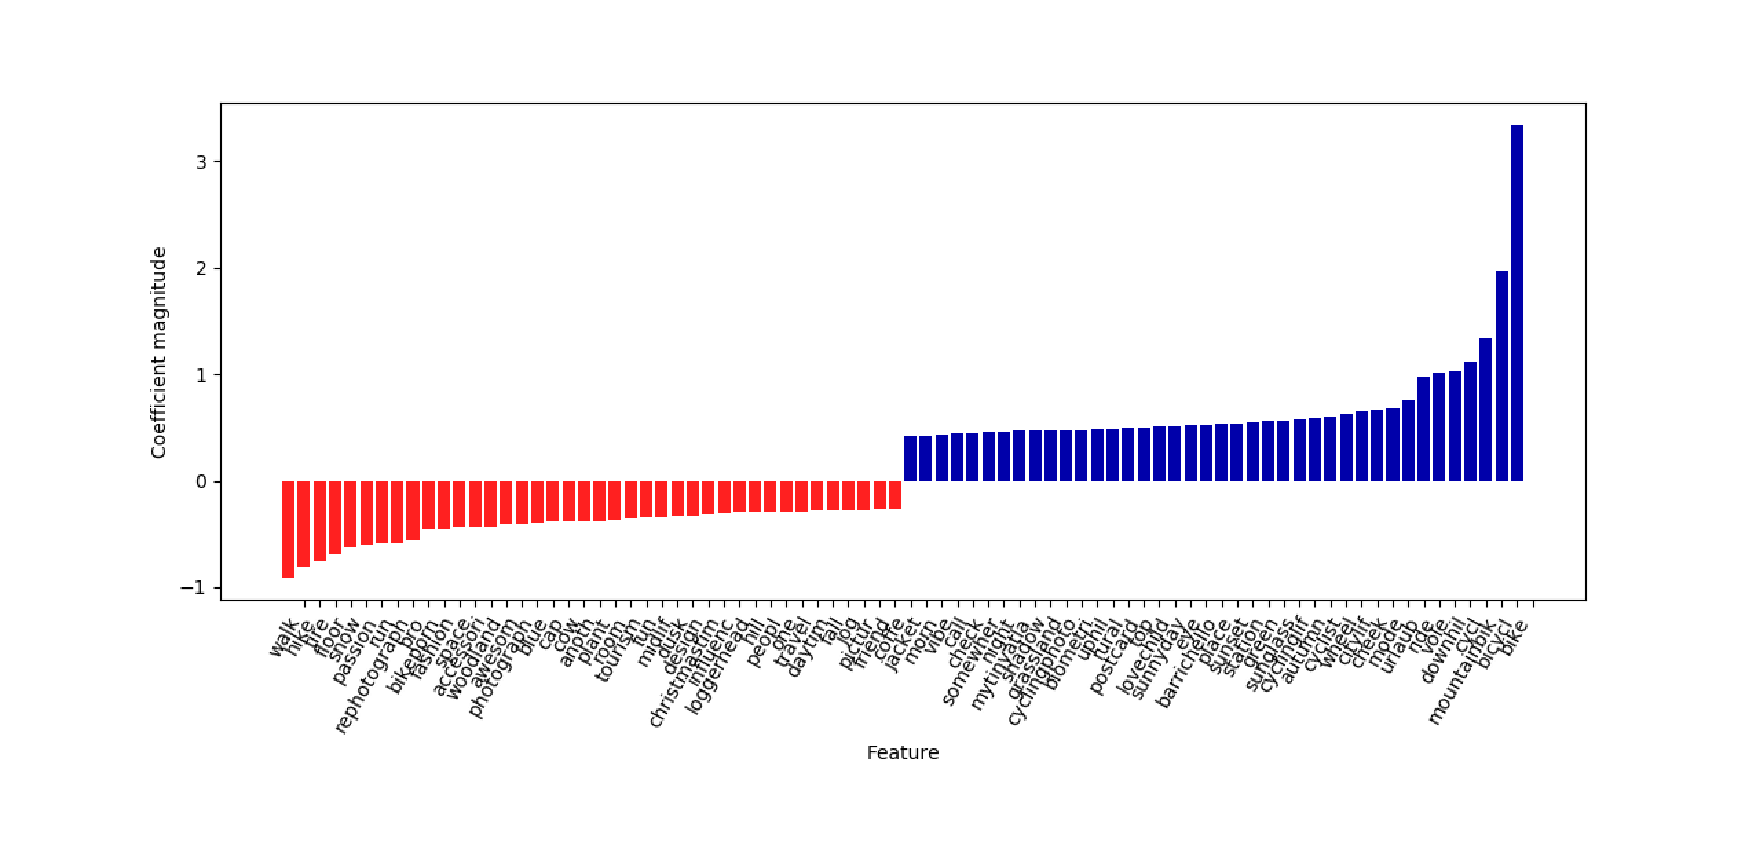
\includegraphics[width=\textwidth]{img/m2_top_40_features_Biking_cropped.pdf}
   \caption{80 most predictive M2-features of the class 'Biking'. Blue features are word-tokens which supports the presence of the corresponding classification. Red features support the opposite. The graphic was created with the \textit{mglearn} Python library provided by \textcite{Guido2016}}
   \label{fig:M2_top40_features_biking}
\end{figure}

\subsection{Model comparison}
The above presented models will subsequently be thoroughly compared in terms of classification specific aspects, hyperparameter behaviour and performance on unseen data (data the models were not trained on). 

\subsubsection*{Hyperparameter interaction}
The effect of different \textit{ngram\_range} settings in combination with varying \textit{C} values of the linearSVC fitting algorithm is illustrated in the heatmaps of figure \ref{fig:heatmaps} for M1 and M2 respectively. The red circles mark the combination with the highest F1-score which corresponds to the best hyperparameter setting of the respective models (see M1 - table \ref{tab:m1_linearSVC_bestParams} and M2 - table \ref{tab:m2_linearSVC_bestParams}). It becomes apparent that the (2, 2) \textit{ngram\_range} as well as the \textit{C} value 0.01 underperform across the board. The F1-scores in the heatmaps are not completely identical to the values found in the corresponding model performance tables \ref{tab:m1_linearSVC_bestscores} (M1) and \ref{tab:m2_linearSVC_bestscores} (M2). This variation is due to randomisation effects of the None media object selection from the database as well as from the model train and test splits (this is partly taken care of by cross-validation).\\

\begin{figure}[h!]
 \begin{subfigure}{0.5\textwidth}
   \centering
   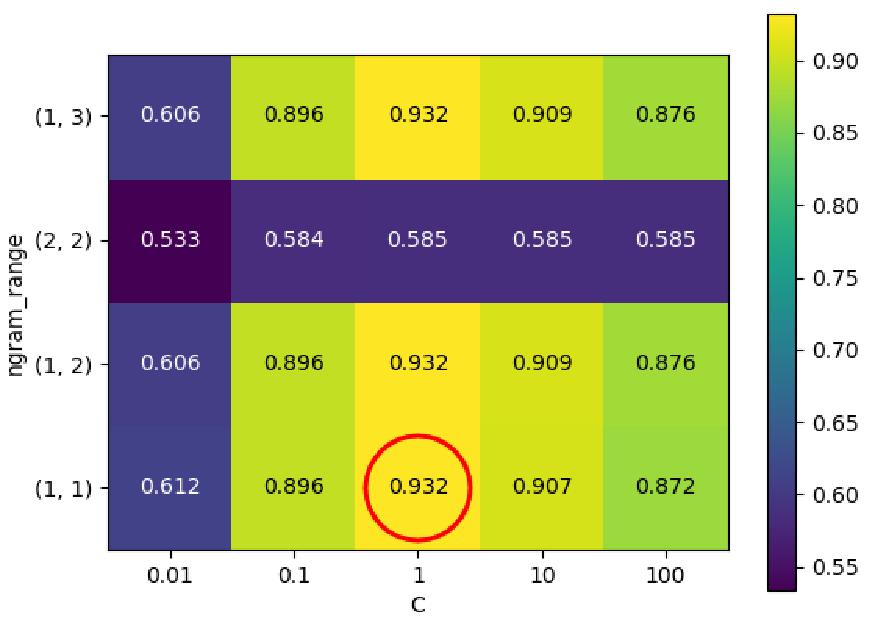
\includegraphics[width=0.9\linewidth]{img/m1_F1_ngram_C_heatmap_w_Circle.pdf}
   \caption{M1 linearSVC}
   \label{fig:m1_heatmap}
\end{subfigure}
\begin{subfigure}{0.5\textwidth}
   \centering
   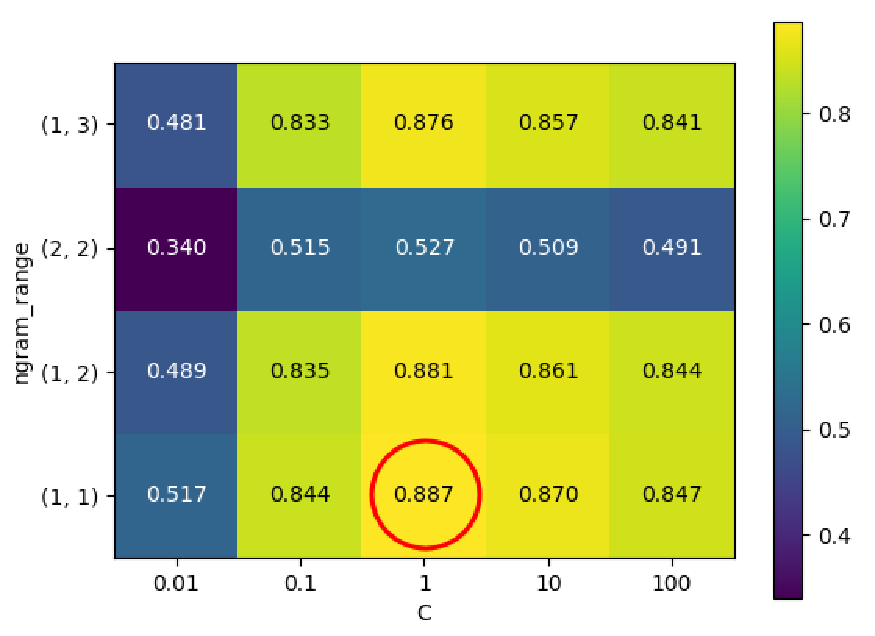
\includegraphics[width=0.9\linewidth]{img/m2_ngram_C_heatmap_new_w_circle.pdf}
   \caption{M2 linearSVC}
   \label{fig:m2_heatmap}
 \end{subfigure}
\caption{These heatmaps shows cross-validated F1-scores of different combinations of the hyperparameters \textit{ngram\_range} and \textit{C} for the model M1 (a) and M2 (b). These graphs were created with the Python library \textit{mglearn} from \textcite{Guido2016}}
\label{fig:heatmaps}
\end{figure}

\texttt{Remark:} If different hyperparameter settings produce the same model performance (F1-score) than the setting which produces fewer features is prioritised due to better generalisation and regularisation capabilities. Regarding figure \ref{fig:m1_heatmap} for instance the \textit{ngram\_range} setting of either (1, 1), (1, 2) or (1, 3) in combination with \textit{C} = 1 all produce a F1-score of 0.932. (1, 1) has been chosen as best hyperparameter configuration due to the lowest feature count.

\subsubsection*{Classification specific F1-scores}
As already seen above M1 performed on the test set with an 10-Fold cross-validated F1-score excluding the None-class of \textbf{0.870} compared to \textbf{0.835} of M2. Figure \ref{fig:m1_m2_class_f1_scores} gives more insight on the classification specific model performances. The worst performances are recorded for both randomForest classifiers. Also the M2 linearSVC picnic class sticks out with a score of 0.48. The actual performance and generalisation potential of both model on 'unseen data' is presented further down.
\begin{figure}[h!]
   \centering
   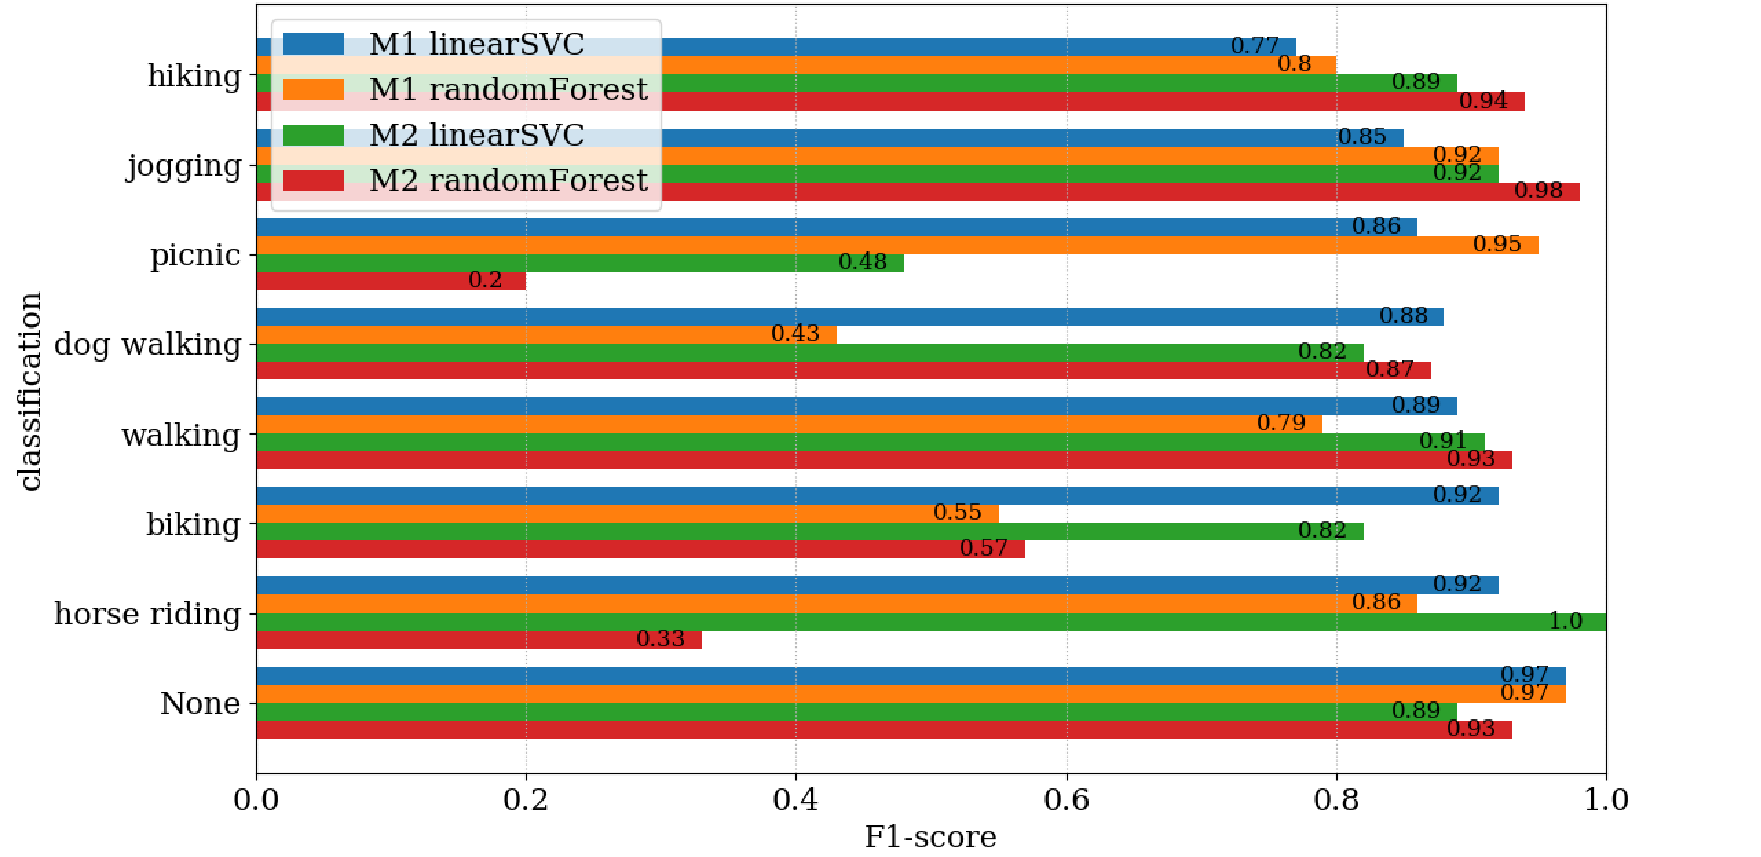
\includegraphics[width=\textwidth]{img/m1_m2_class_f1_scores_bigger_font.pdf}
   \caption{Overview of the classification specific 10-Fold cross-validated F1-scores of the linearSVC and randomForest fitting algorithm of M1 and M2}
   \label{fig:m1_m2_class_f1_scores}
\end{figure}

\subsubsection*{Final model scores}
In the end both models were trained on the entire training's dataset which resulted in the following final performance scores visible in table \ref{tab:m1_m2_linearSVC_final_scores}. This step is important to generate a finalised model that is eventually trained on as much training's data as possible. Keeping a data aside for model testing is no longer necessary because the most well performing hyperparameter configuration is already determined.\\
It can be noted at this point that the best M1 and M2 performance yielded similar feature counts during testing (626 and 775 respectively) as well as after training it on the entire dataset (845 and 958 respectively). Also, contradicting to the already presented model performances during model-tuning M2 now performs slightly better than M1. Possible reasons for this observation will be discussed in the section \ref{disussion_model_performance}.

\begin{table}[h]
\begin{center}
\caption{linearSVC 10-Fold cross-validated final performance scores of M1 and M2 while being fitted according to the entire training's dataset available.}\vspace{1ex}
\label{tab:m1_m2_linearSVC_final_scores}
\begin{tabular}{cccccc}\hline
Model & Accuracy & Precision & Recall & F1 & F1 (without None-class) & Features\\ \hline
M1 & 0.984 & 0.984 & 0.984 & 0.984 & 0.967 & 845\\
M2 & 0.991 & 0.991 & 0.991 & 0.991 & 0.993 & 958\\ \hline
\end{tabular}
\end{center}
\end{table}

\subsubsection*{Precision on unseen data} \label{precision_unseen_data}
This section will present the model performances on new data. All Instagram and Flickr media objects of the Canton of Zug on which these results are based were excluded from the M1 and M2 model training.\\
Two separate predictions per model were performed on the media objects contained in the following two database-tables (database overview see section \ref{database_setup}):

\begin{itemize}
    \item \texttt{media\_objects\_unionzug\_instagram} \item \texttt{media\_objects\_cantonzug\_flickr}
\end{itemize}

One time the final text-string provided for the prediction was constructed by concatenating the processed text-data and the image labels of a given media object. The second time the final text-string only contained the processed text-data.\\

The model performance evaluation was done manually by the author. 100 media objects (if available) per class, per prediction-mode and per model were evaluated for True Positive (TP) or False Positive (FP) predictions. Only the model precision can be calculated with this information. An estimate for the recall over all classes was made based on the share of media objects that were correctly classified (except the None-class) in relation to the total amount of media objects present. In other words, how many media objects that actually contained NBRAs were also identified as such? This information is important because e.g. a model with 95\% precision that only identifies 20\% of media objects containing NBRAs is still not practical. This approximation was calculated in the following way:

\begin{equation}
\label{equation_share_TP}
\frac{\sum_{class=1}^{7}(precision_{class}  * n^{total}_{class})}{n^{total}_{dataset}} * 100
\end{equation}
   
where the class-specific model precision (\textit{precision}\textsubscript{class}) is based on the manual evaluation of 100 media objects of that class which can be a subset of the total amount of predicted media objects of that class by the model.

\paragraph*{Model 1}
The best M1 precision of \textbf{0.764} was recorded for the media objects of the SMP Flickr while the parsed text-string excluded image labels (see table \ref{tab:m1_actual_precision}). Predicting new data without image labels across both SMPs yields accordingly an average precision score of \textbf{0.748}.\\
While the M1 precision differences between the two SMPs Instagram and Flickr were not significant on a 5\% level, the recorded differences between the inclusion and exclusion of image labels were significant.

\begin{table}[h!]
\begin{center}
\caption{M1 NBRA precision on unseen data}\vspace{1ex}
\label{tab:m1_actual_precision}
\begin{tabular}{c|cc?cc}\hline
SMP & +image labels & -image labels & $\bar{x}$ & ratio\\ \hline
Instagram & 0.664 & 0.732 & 0.698 & 0.907\\
Flickr & 0.634 & 0.764 & 0.699 & 0.830\\
\Xhline{2\arrayrulewidth}
$\bar{x}$ & 0.649 & 0.748 \\
%\cline{1-3}
ratio & 1.047 & 0.958  
\end{tabular}
\end{center}
\end{table}

The incorporation of image labels into the text-string results in an increase of overall and true positive predictions for both SMPs (see table \ref{tab:m1_actual_recall}).
In the case of Instagram the inclusion and exclusion of image labels results in a total of \textbf{668} and \textbf{384} NBRA-identifications which corresponds to 5.67\% and 3.26\% respectively of the 11'777 media objects in the database table \texttt{media\_objects\_unionzug\_instagram}.
In the case of Flickr the inclusion and exclusion of image labels results in a total of \textbf{273} and \textbf{67} NBRA-identifications which corresponds to 4.25\% and 1.77\% respectively of the 3'790 media objects in the database table \texttt{media\_objects\_cantonzug\_flickr}.\\
Therefore, the best performing final text-string format which excludes image labels results in a total of \textbf{451} (extrapolation based on the calculated precision on 100 media objects per class) true positive NBRA media objects across both SMPs. 

\begin{table}[h!]
\begin{center}
\caption{Share of correctly classified NBRA media objects by M1 (except the None-class) in relation to the entire dataset (according to listing \ref{equation_share_TP})}\vspace{1ex}
\label{tab:m1_actual_recall}
\begin{tabular}{ccc?cc}\hline
SMP & +image labels & -image labels & $\bar{x}$ & ratio\\ \hline
Instagram & 5.67\% & 3.26\% & 4.47\% & 1.74\\
Flickr & 4.25\% & 1.77\% & 3.01\% & 2.40\\
\Xhline{2\arrayrulewidth}
$\bar{x}$ & 4.96\% & 2.52\% \\
ratio & 1.33 & 1.84 
\end{tabular}
\end{center}
\end{table}

\paragraph*{Model 2}
The best M2 precision of \textbf{0.776} was recorded for the media objects of the SMP Instagram while the parsed text-string included image labels (see table \ref{tab:m2_actual_precision}). Predicting new data with image labels across both SMPs yields accordingly an average model performance of \textbf{0.749}.\\
While the M2 precision differences between the two SMPs Instagram and Flickr were not significant on a 5\% level, the recorded differences between the inclusion and exclusion of image labels were significant.\\


\begin{table}[h!]
\begin{center}
\caption{M2 NBRA precision on unseen data}\vspace{1ex}
\label{tab:m2_actual_precision}
\begin{tabular}{ccc?cc}\hline
SMP & +image labels & -image labels & $\bar{x}$ & ratio\\ \hline
Instagram & 0.776 & 0.691 & 0.734 & 1.123\\
Flickr & 0.721 & 0.753 & 0.737 & 0.958\\
\Xhline{2\arrayrulewidth}
$\bar{x}$ & 0.749 & 0.722\\
ratio & 1.076 & 0.918   
\end{tabular}
\end{center}
\end{table}

The incorporation of image labels into the final text-string results in a significant increase of overall and true positive predictions for both SMPs (see table \ref{tab:m2_actual_recall}).
In the case of Instagram the inclusion and exclusion of image labels results in a total of \textbf{710} and \textbf{137} NBRA-identifications which corresponds to 6.03\% and 3.63\% respectively of the 11'777 media objects in the database table \texttt{media\_objects\_unionzug\_instagram}. In the case of Flickr the inclusion and exclusion of image labels results in a total of \textbf{227} and \textbf{82} NBRA-identifications which corresponds to 5.99\% and 2.16\% respectively of the 3'790 media objects in the database table \texttt{media\_objects\_cantonzug\_flickr}.\\
Therefore, the best performing final text-string format which includes image labels results in a total of \textbf{937} (extrapolation based on the calculated precision on 100 media objects per class) true positive NBRA media objects across both SMPs. 

\begin{table}[h!]
\begin{center}
\caption{Share of correctly classified NBRA media objects by M2 (except the None-class) in relation to the entire dataset (according to listing \ref{equation_share_TP})}\vspace{1ex}
\label{tab:m2_actual_recall}
\begin{tabular}{ccc?cc}\hline
SMP & +image labels & -image labels & $\bar{x}$ & ratio\\ \hline
Instagram & 6.03\% & 3.63\% & 4.83\% & 1.66\\
Flickr & 5.99\% & 2.16\% & 4.08\% & 2.77\\
\Xhline{2\arrayrulewidth}
$\bar{x}$ & 6.01\% & 2.90\% \\
ratio & 1.00 & 1.68 
\end{tabular}
\end{center}
\end{table}

\paragraph*{Summary}
M1 and M2 showed both the best performance if the parsed data for prediction (final text-string) was in the form the model was originally trained.\\
The model precision was less dependant on the SMP the media objects originated from but rather if image labels were parsed or not.\\
The best observed precision of M2 with \textbf{0.776} (SMP average: 0.749) was only slightly better than the \textbf{0.764} of M1 (SMP average: 0.748). Strong differences were registered in the percentage of correctly classified media objects in relation to the entire dataset which lay at \textbf{6.01\%} for M2 but only at \textbf{2.52\%} for M1.
M2 with a slightly higher precision yielded (937-451=)486 more true positive NBRA-predictions than M1 which resolves to an \textbf{increase by factor two}. Therefore, M2 predicted less False Negatives (FN) which concludes that M2 also possess a higher recall score than M1 and generalises better on new data.

\section{Media object languages}
One assumption that was made earlier stated that the training's data from Zurich and the media objects from Zug share a similar written language by their author base. This would legitimise the usage of training's data that did not originate from the same region as the region the model would later be applied to.\\
To investigate on that assumption the five actively detected Instagram media object languages of both regions were compared (see figure \ref{fig:det_languages}) with a paired two sample t-test for means. The result showed on a significance level of 5\% that the probability that T is smaller or equal to t is 0.56 and therefore smaller than t\textsubscript{crit} of 2.78. Therefore, the null-hypothesis \textit{H\textsubscript{0}} (no difference present) cannot be rejected and the written languages of both areas are with high certainty of similar composition.

\begin{figure}[h!]
   \centering
   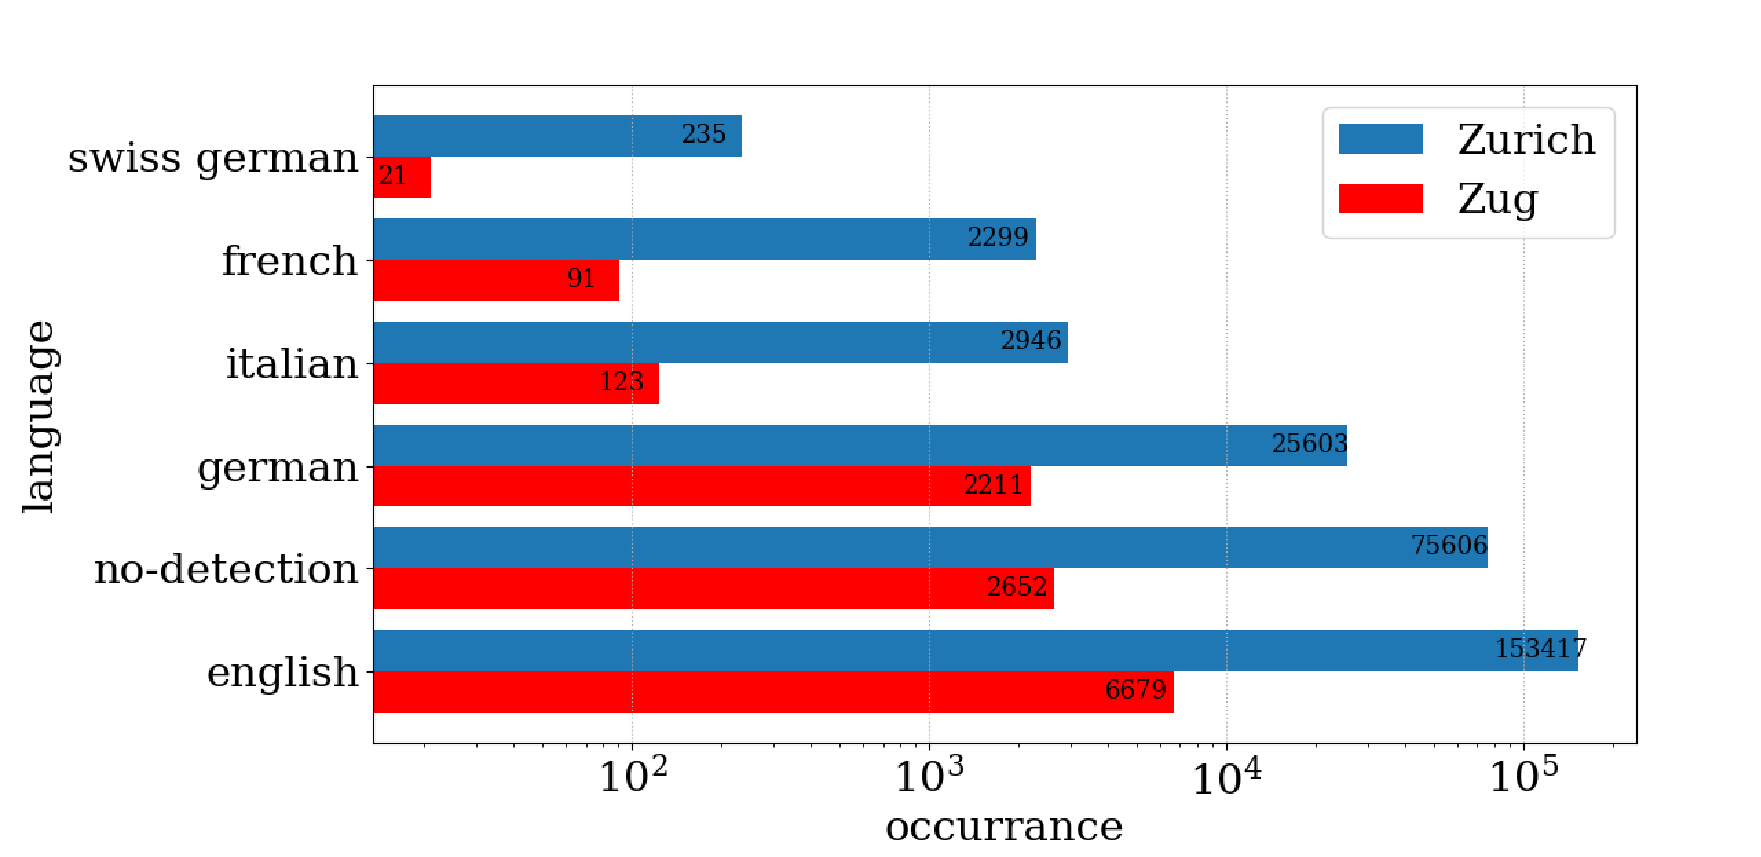
\includegraphics[width=\textwidth]{img/det_languages_bigger_font.pdf}
   \caption{Comparison between detected languages of Instagram media objects originating from the Canton of Zug and Zurich}
   \label{fig:det_languages}
\end{figure}

\texttt{Remark:} Often times hashtags remain written in English due to their comprehensive meaning and purpose to connect media objects of similar content. Due to the big share hashtags normally have on the entire text corpus the language detection tends to identify a media object language as English above others.

\section{Ground truth evaluation}
The following subsections will cover the results from the \textit{in-situ} ground truthing through passive observations and the 52 interviews over the three different locations 'Br\"uggli', 'R\"ossliwiese' and 'Schattenw\"aldli' (see figure \ref{fig:locations_ground_truthing}) in the research area.

\texttt{Remark:} The entire data presented in the following subsections is available on the enclosed CD to this thesis. This includes the actual transcript-data from the passive observation and the interviews (see chapter \ref{CD_content}).

\subsection{Passive observation analysis}
The passive NBRA-observation was performed by an assistant of the author. The thereby collected data is visible in figure \ref{fig:passive_observation} and shows the recorded NBRAs based on location sorted from left to right by decreasing observation frequency. Walking and hiking were by far the most recorded classes which corresponds to the interviews results visible in figure \ref{fig:interview_activities}. These two classes were merged due to differentiation difficulties just by observation and the demanded recording speed. 'Biking' follows second with a strong signal in the location 'Br\"uggli' and no occurrence at 'R\"ossliwiese'. Third is 'jogging' shortly followed by 'dog walking' which have roughly the same occurrence frequency distribution across all three locations.

\begin{figure}[h!]
   \centering
   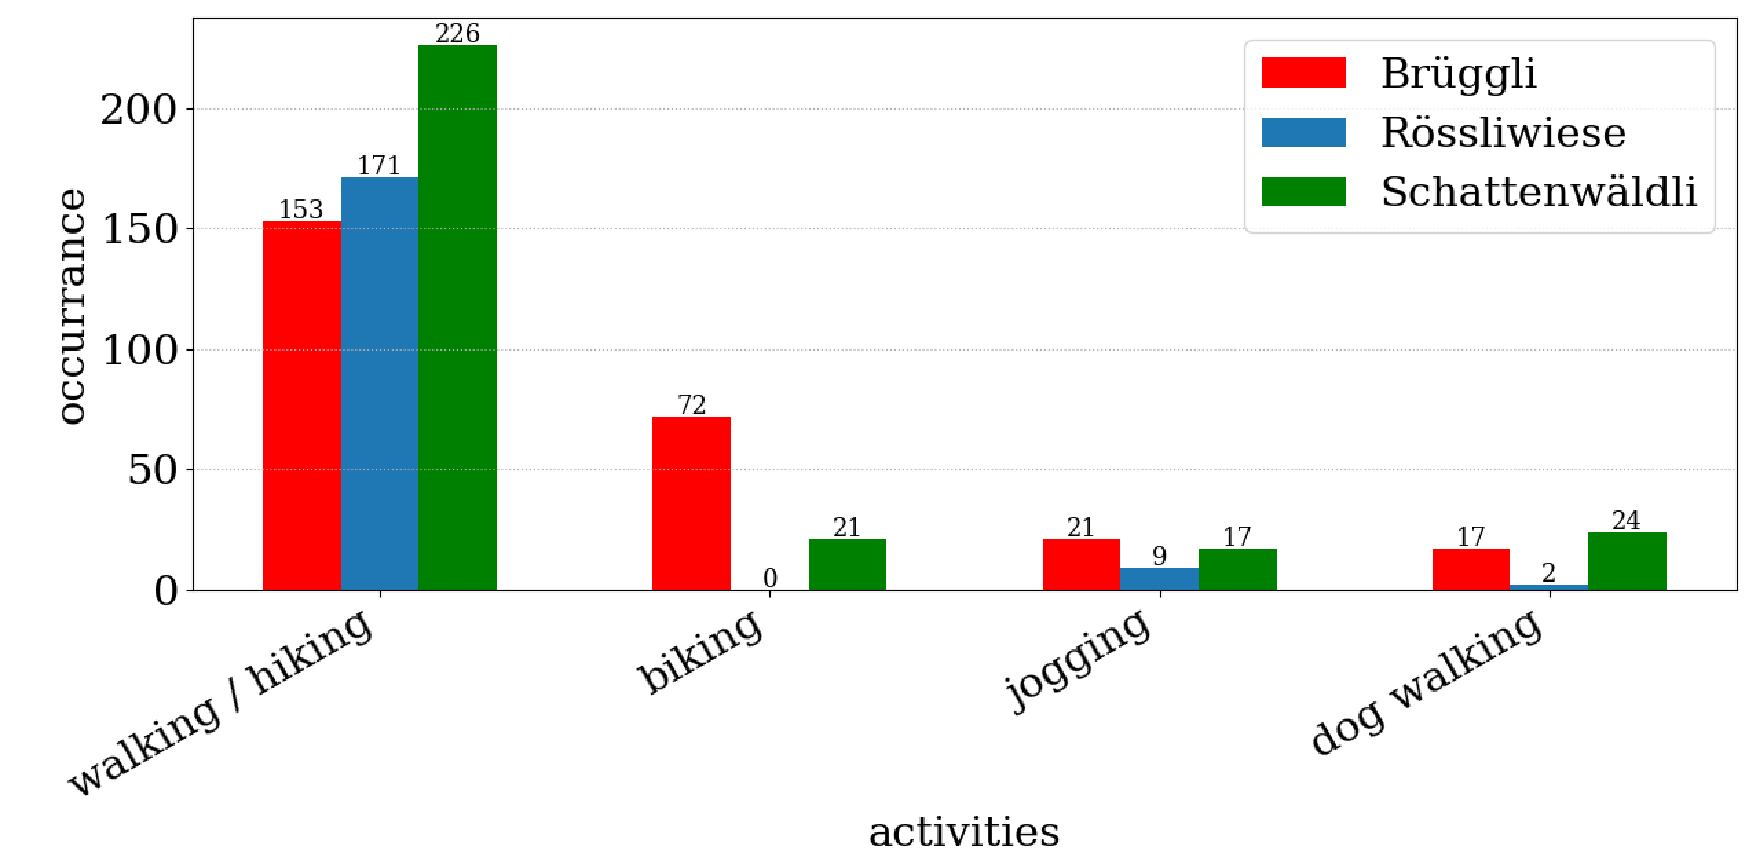
\includegraphics[width=\textwidth]{img/passive_observations.pdf}
   \caption{NBRA-occurrence according to the passive observation performed in the three locations listed in the legend}
   \label{fig:passive_observation}
\end{figure}

\subsection{Interview analysis}

\subsubsection*{Visitation motivations}
The top eight motivations or reasons the interviewees mentioned why they visited a given location are displayed in figure \ref{fig:interview_visitation_motivation} sorted from left to right in descending order. According to the results plays \textit{geographic closeness} a dominant role how people choose their recreation location. If a lake was present it was also frequently mentioned as a strong driver that attracts people for NBRAs. The term \textit{sport} was solely mentioned for the location 'Schattenw\"aldli', the terms \textit{shopping}, \textit{low traffic} and \textit{sunset} exclusively for the location 'R\"ossliwiese' and the term \textit{topography} for the location 'Br\"uggli'.

\begin{figure}[h!]
   \centering
   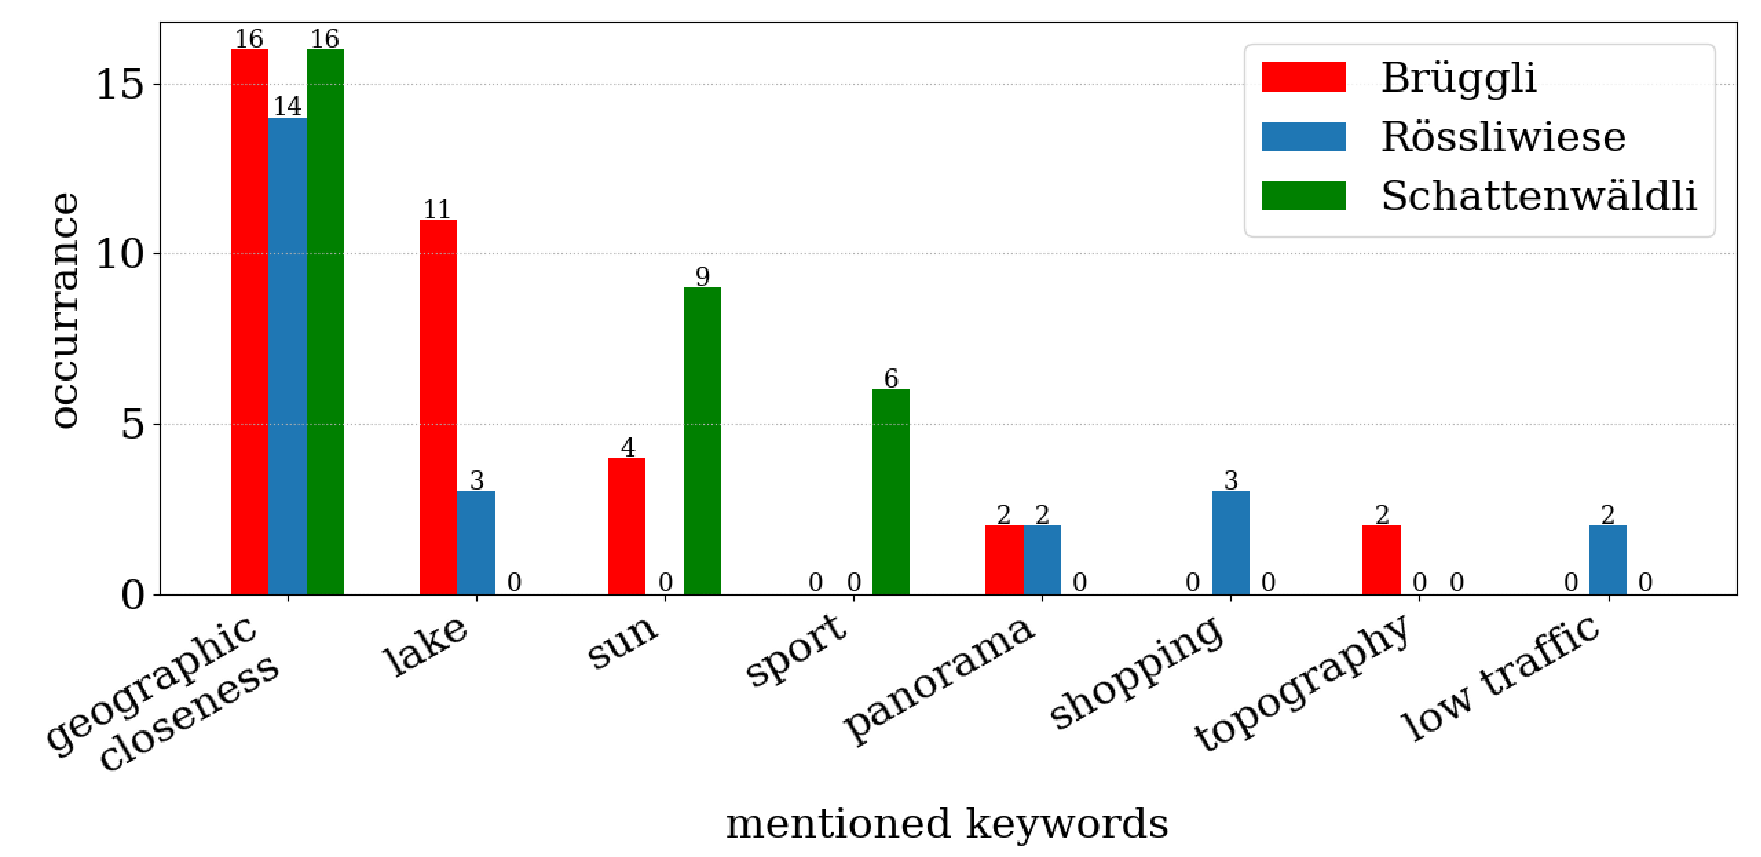
\includegraphics[width=\textwidth]{img/interview_keywords.pdf}
   \caption{Frequency of drivers mentioned by 52 interviewees for visiting one of the three locations listed in the legend.}
   \label{fig:interview_visitation_motivation}
\end{figure}

\subsubsection*{Recorded NBRAs}
Figure \ref{fig:interview_activities} corresponds to figure \ref{fig:passive_observation} and shows similarly the performed NBRAs. This time the descriptive term came from the interviewees themselves which explains why the differentiation between the classes 'walking' and 'hiking' is again established. 'Walking' still holds the biggest share across all three locations. 'Biking' follows again second and was recorded everywhere but in the location 'R\"ossliwiese' to which 'relaxing' was exclusive. Third comes 'hiking' which was only found on the mountain location 'Schattenw\"aldli'. The NBRA 'swimming' was not actively performed at the time of the interviews but it was instead mentioned by the interviewees as a regular summer activity at the location 'Br\"uggli'.

\begin{figure}[h!]
   \centering
   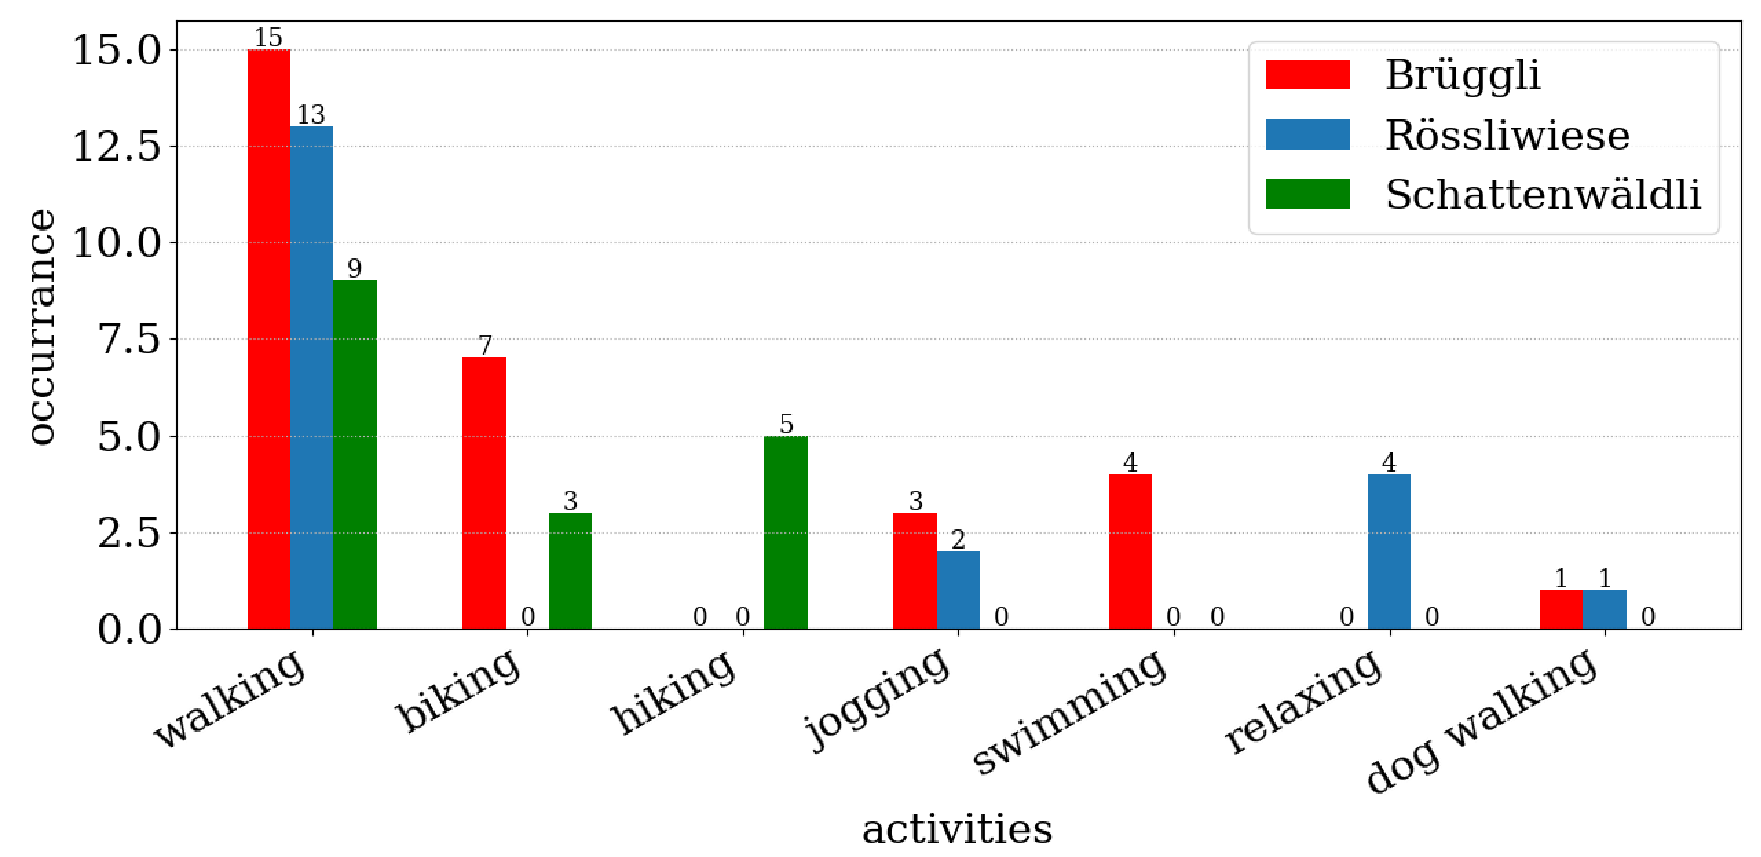
\includegraphics[width=\textwidth]{img/interview_activities.pdf}
   \caption{NBRA-occurrence according to the 52 performed interviews in the three locations listed in the legend}
   \label{fig:interview_activities}
\end{figure}

\subsubsection*{Popularity of social media platforms }
One main part of the interviews next to the information gain related to the performed NBRAs was dedicated to the interviewee's social media usage and engagement. Figure \ref{fig:interview_SMP} visualises the recorded occurrences where interviewees confirmed having an account on one of the given SMPs. Instagram and Facebook are by far the most widespread SMPs that were registered. LinkedIn follows third with less than half of the mentions of first or second place. Many interviewees mentioned the (sometimes forced) requirement of a LinkedIn account for their professional life. A surprisingly low occurrence is registered for Twitter. STRAVA through being a specialised SMP was only mentioned once. Interestingly Flickr was not mentioned once during all 52 interviews.

\begin{figure}[h!]
   \centering
   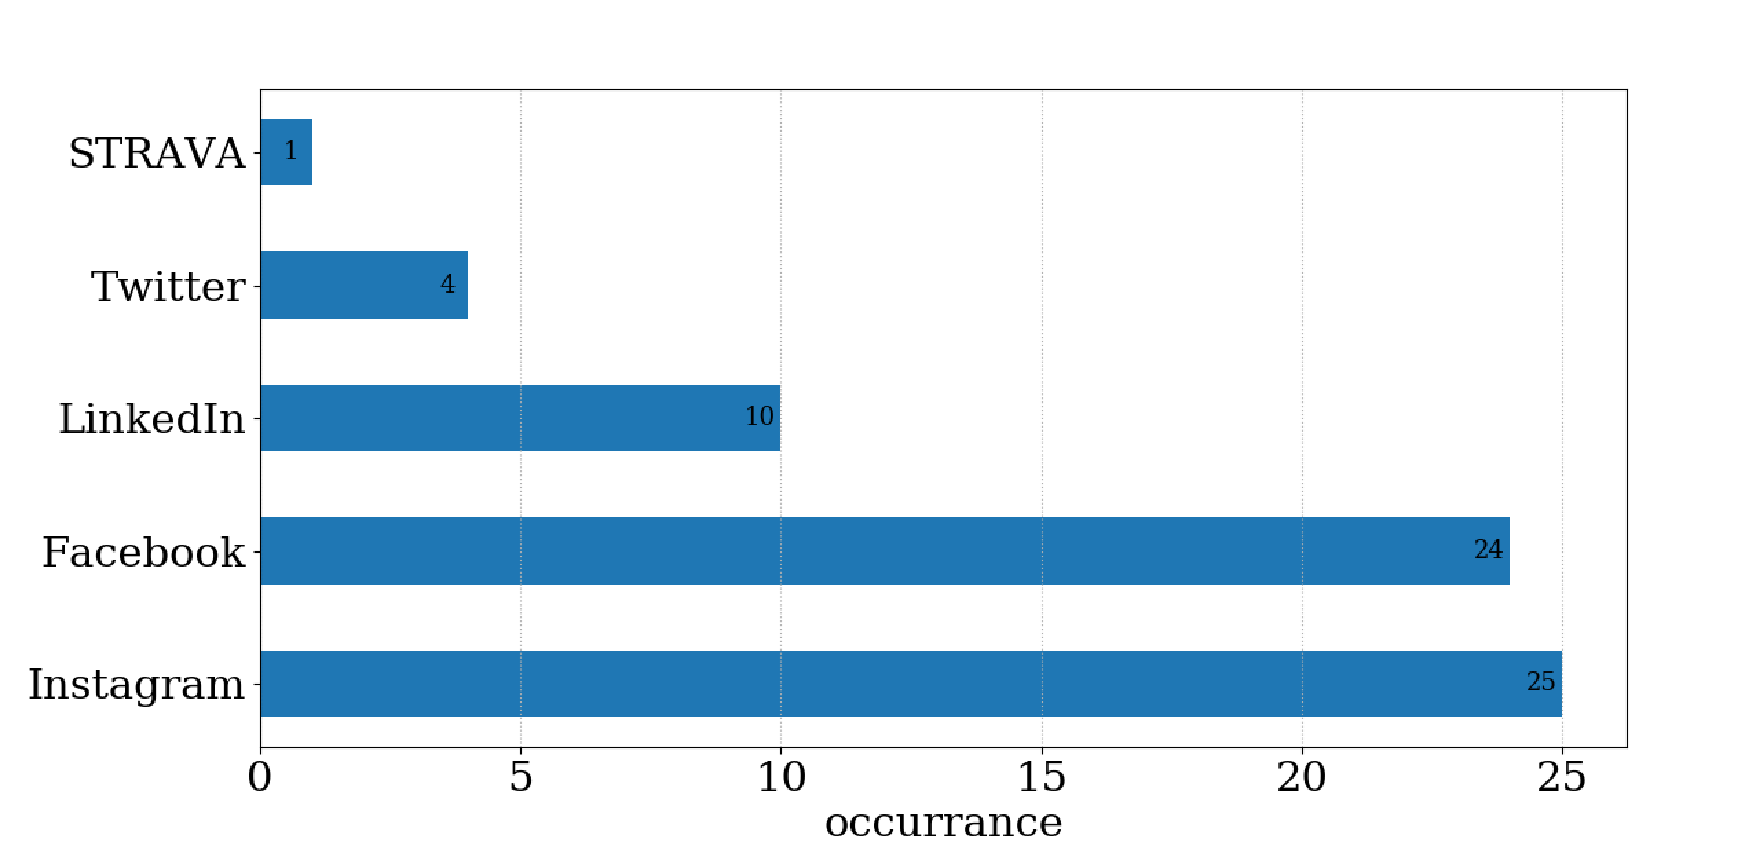
\includegraphics[width=\textwidth]{img/interview_socialmedia_bigger_font.pdf}
   \caption{Deviated SMP popularity according to confirmed profiles of 52 interviewees}
   \label{fig:interview_SMP}
\end{figure}

\subsubsection*{Relationship between age and social media presence}
Insight on dominantly represented ages groups in social media data can be drawn from figure \ref{fig:interview_age_SMP}. According to the 52 conducted interviews are the most active people on SMPs between the age of 21 and 30 (red bars indicating participation). The age group of 61 to 100 on the other hand has not one recorded social media user. The red and blue line in figure \ref{fig:interview_age_SMP} represent the linear regression lines of the corresponding datasets. Their intersection at roughly age 50 indicates the transition between SMP usage and absence. Instagram and Facebook make out the biggest share of these records as already seen in figure \ref{fig:interview_SMP}.

\begin{figure}[h!]
   \centering
   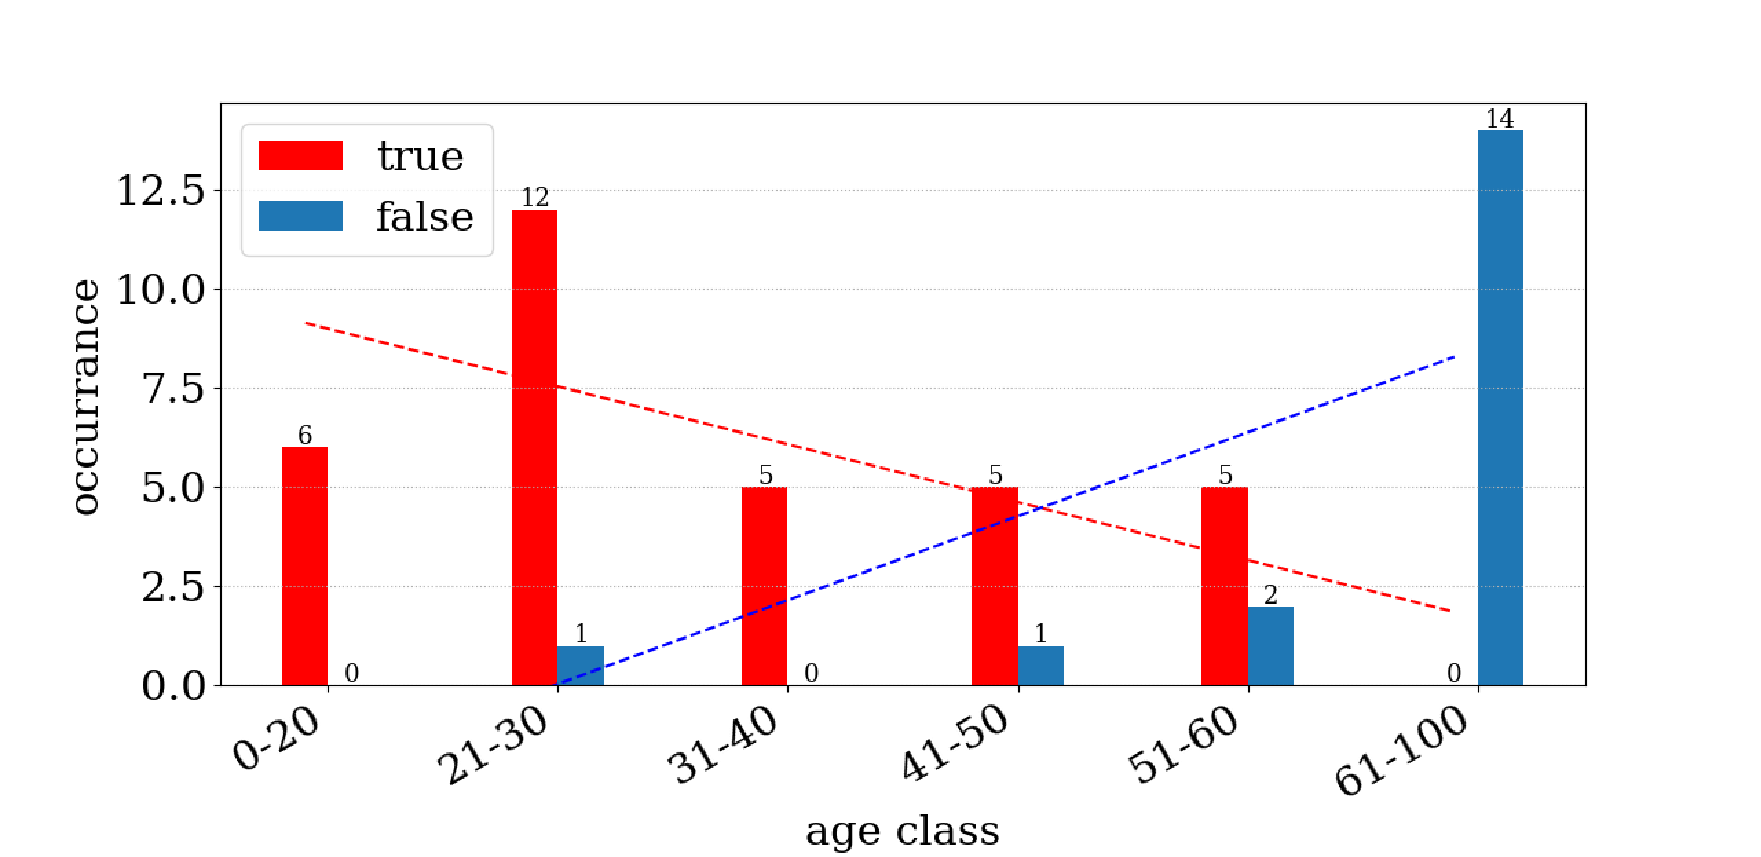
\includegraphics[width=\textwidth]{img/interview_socialmedia_age_bigger_font.pdf}
   \caption{Share per age class of social media users (true) and the once that do not use it (false). The red and blue line represent the linear regression of their corresponding dataset.}
   \label{fig:interview_age_SMP}
\end{figure}

\section{Spatial distribution of model predicted NBRAs}
This section will present the maps which resulted from the M2 NBRA-predictions on both Instagram and Flickr media objects from the Canton of Zug. The maps in figure \ref{fig:map_cluster_1} and figure \ref{fig:map_cluster_2} show the NBRAs spatial distribution in parallel comparison between the two SMPs. The amount of M2 predictions per classification and SMP are listed in table \ref{tab:amount_class_NBRAs} as well as in the maps themselves as \textit{feature count}.

\begin{table}[h!]
\begin{center}
\caption{Amounts of M2 classified media objects that contain NBRAs}\vspace{1ex}
\label{tab:amount_class_NBRAs}
\begin{tabular}{cccc}\hline
Class & Instagram & Flickr & Total\\ \hline
Hiking & 231 & 126 & 357\\
Walking & 265 & 55 & 320\\
Dog walking & 143 & 16 & 159\\
Biking & 95 & 51 & 146\\
Jogging & 85 & 19 & 104\\
Horse riding & 37 & 6 & 43\\
Picnic & 23 & 6 & 29\\
 & & & \\
None & 10'898 & 3'511 & 14'409\\
\hline
\end{tabular}
\end{center}
\end{table}

As mentioned in section \ref{instagram_location_tag} Instagram locations can be user generated and are often general descriptions of the area at hand. This results in media objects being snapped to the same point on the map which leads to a lower spatial resolution. For further illustration a comparison between the two SMPs in regards to location numbers is made:
There are \textbf{152} unique Instagram locations of which the top three are named 'Zug' with 1'970, 'Canton of Zug' with 1'590 and 'lake Zug' with 400 associated media objects.
The processed Flickr dataset on the other hand consists of \textbf{1'144} unique locations of which the top three are named 'Baarerstrasse 12' with 112, 'Bahnhofsplatz' with 84 and 'Landsgemeindeplatz' with 69 associated media objects. This additional geo-information in form of an address is not provided by the Flickr API by default but rather through the Google Geocoding API as stated in section \ref{geocoding_api}. \\
One has to keep in mind that the processed Flickr dataset holds only roughly a third of the media objects compared to the processed Instagram dataset in the area of interest while possessing 7.5 times as many unique locations. 

\begin{figure}[h!]
   \centering
   \includegraphics[width=\textwidth,height=\textheight,keepaspectratio]{img/map_cluster_1.pdf}
   \caption{Part 1 - Spatial NBRA-occurrences in the Canton of Zug based on M2 predictions which were conducted on text strings containing processed text-data and image labels from the Instagram / Flickr media objects.}
   \label{fig:map_cluster_1}
\end{figure}

\begin{figure}[h!]
   \centering
   \includegraphics[width=\textwidth,height=\textheight,keepaspectratio]{img/map_cluster_2.pdf}
   \caption{Part 2 - Spatial NBRA-occurrences in the Canton of Zug based on M2 predictions which were conducted on text strings containing processed text-data and image labels from the Instagram / Flickr media objects.}
   \label{fig:map_cluster_2}
\end{figure}

\subsection{Comparison to ground truth}
The modelled output of M2 (see maps in figure \ref{fig:map_cluster_1} and figure \ref{fig:map_cluster_2}) was visually compared to the ground truth visible in figure \ref{fig:passive_observation} and figure \ref{fig:interview_activities} to further evaluate the model's plausibility.

\paragraph*{Biking}
The model predicts a strong occurrence of biking in the area of 'R\"ossliwiese' where the ground truthing consisting of the passive observation and the interviews did not record a single sighting (to the knowledge of the author: biking is not prohibited there and normally performed regularly).\\
In the area of 'Schattenw\"aldli' and 'B\"uggli' the ground truth recorded a moderate to strong occurrence of (mountain-)bikers. Only the former is also registered by the model. 

\paragraph*{Hiking}
'Schattenw\"aldli' is according to the interviews the only location of the three where the NBRA 'hiking' is performed. The model shows also a strong signal of 'hiking' in the mountainous region. Inconsistency lies in the as 'hiking' classified media objects located in the urban area of the city of Zug.

\paragraph*{Jogging}
The maps as well as the ground truth show moderate congruent signals in all three locations.

\paragraph*{Walking}
M2 records a predominant signal in the urban areas over the mountainous areas. Especially the lake side is strongly represented which coincides with the interviewee given motivation 'lake' listed in figure \ref{fig:interview_visitation_motivation} as well as with the high recorded interview 'walking' frequency in the locations 'Br\"uggli' and 'R\"ossliwiese' visible in figure \ref{fig:interview_activities}. Flickr recorded one obvious false occurrence of 'walking' on the lake of Zug which resembles a media object with the title "walk on water" of a stand-up paddler.

\paragraph*{Picnic}
The ground truth does not yield any information on that classification.

\paragraph*{Dog walking}
The NBRA 'dog walking' is according to the ground truth performed in all three locations in a comparably low frequency similar to 'jogging'. The M2 Instagram-data shows a signal densification in the urban area of the city of Zug whereas the Flickr-data shows a homogeneous distribution without any clear hot-spots.

\paragraph*{Horse riding}
The ground truth does not yield any information on that classification.

\paragraph*{None} The M2 'None' classification signal shows as expected a homogeneous distribution (especially the Flickr-data with the higher spatial resolution) without any visible patterns. Because non-NBRAs were not actively recorded during the ground truthing a direct comparison cannot be made.

\paragraph*{Summary}
Essentially predicted the model spatial patterns which coincide with the available ground truth data. An exception is the classification 'hiking' which shows discrepancy and overlaps with the classification 'walking'.  This observation might be related to superordinate Instagram locations positioned in the urban areas. Refer to section \ref{discussion_rec_bias} in the discussion for further insight on this topic. 


\subsection{Comparison to Foursquare}
The SMP Foursquare holds records of categorised infrastructure (venues). The map in figure \ref{fig:map_foursquare_comparison} visualises 378 Foursquare venues of the category \textit{Outdoor \& Recreation} in relation to the M2 predicted NBRA-occurrences in the Instagram and Flickr dataset of the Canton of Zug.\\
For reasons of time a spatial similarity analysis between the datasets could not be conducted. Instead a visual evaluation shall give insight on the spatial concordance. The NBRA-types were not analysed individually due to the considerable overlap in supporting infrastructure between them. \\
The map shows a plausible densification of venues in or near urban areas. The occurrences of NBRAs and venues seem to match spatially quite well which suggests that the supporting infrastructure is already efficiently allocated to fit the peoples recreation needs. This claim has to be further analysed with an appropriate statistical evaluation. \\
The Foursquare dataset in conjunction with the modelled NBRA occurrences shall moreover give agencies a tool to plan the allocation of sport and recreation related infrastructure in case of rezoning or land conversion.

\begin{figure}[h!]
   \centering
   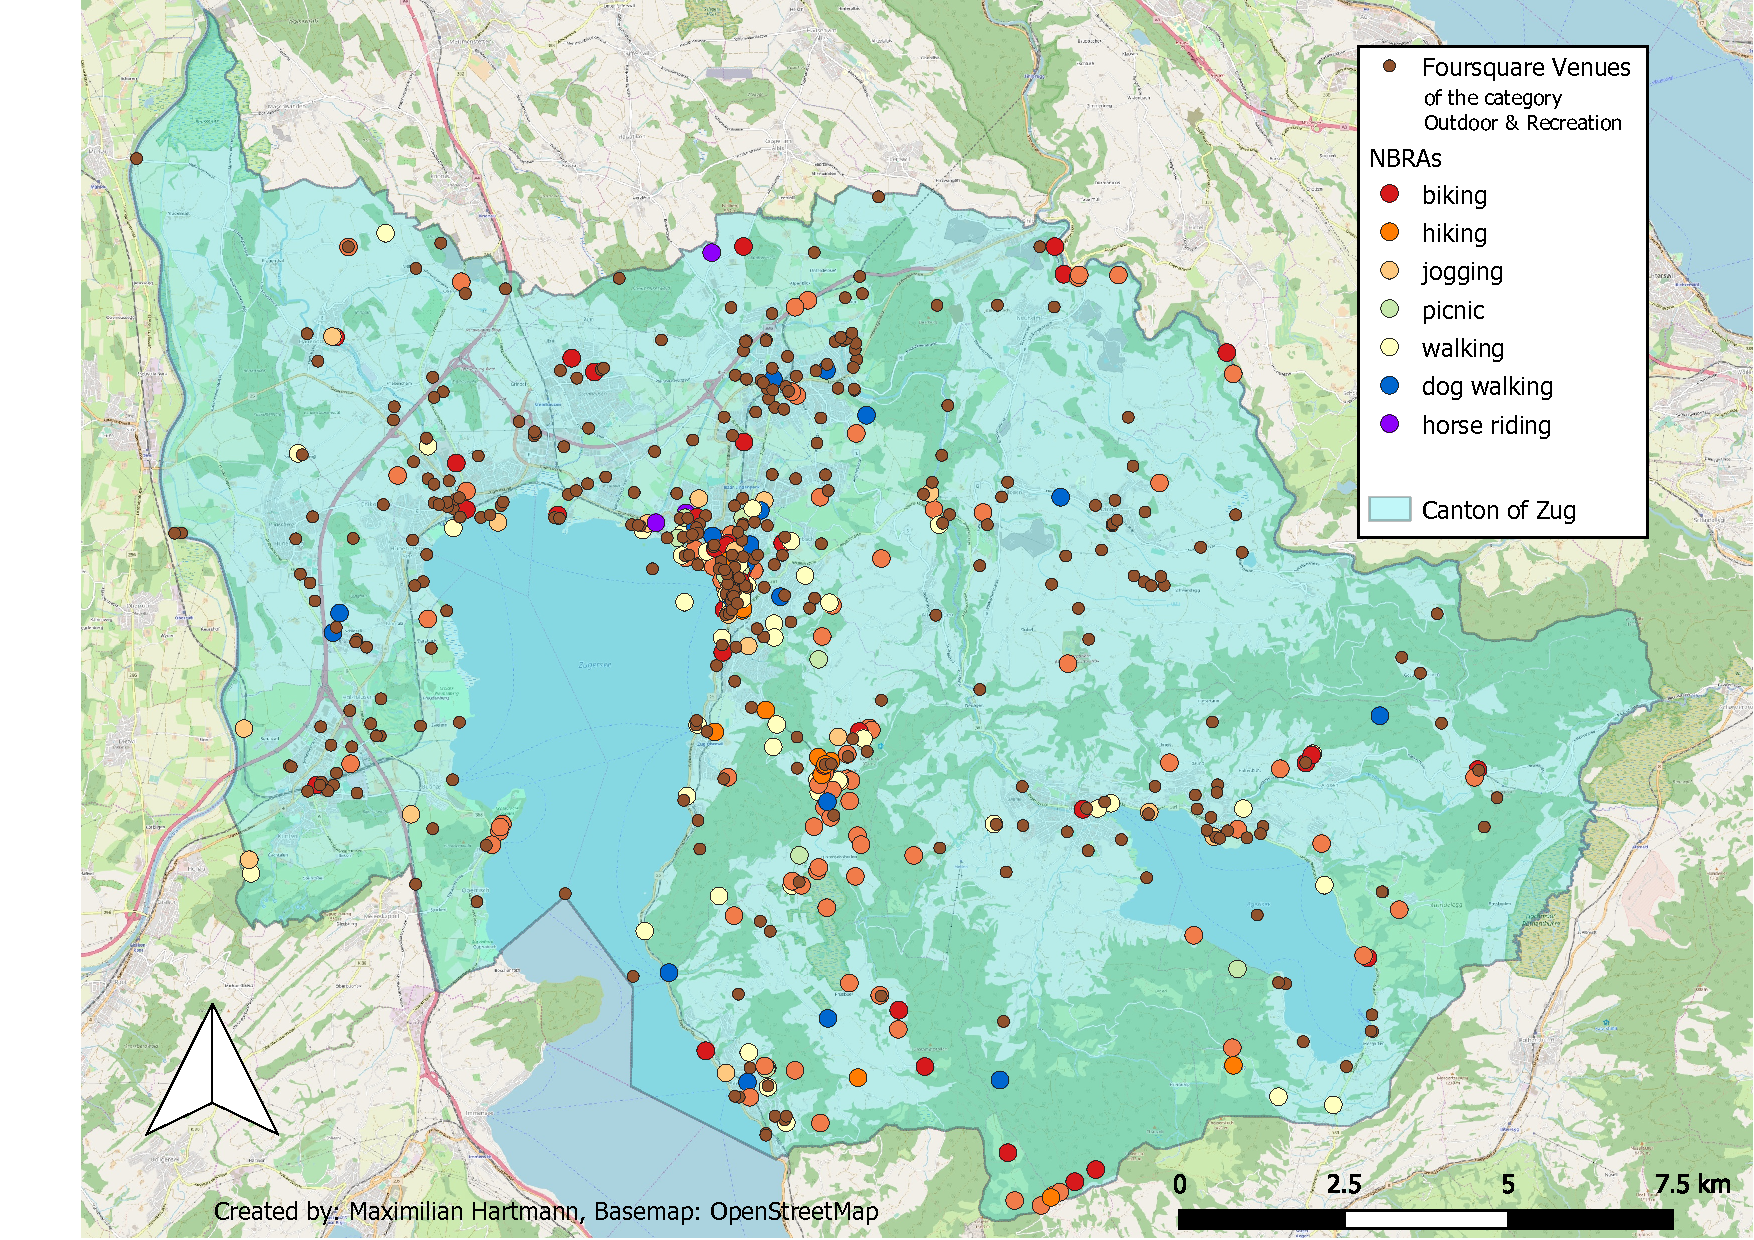
\includegraphics[width=\textwidth,height=\textheight,keepaspectratio]{img/foursquare_comparison_cropped.pdf}
   \caption{Locations of all 378 Foursquare venues of the category \textit{Outdoor \& Recreation} in relation to the M2 predicted spatial NBRA-occurrence of the SMPs Instagram and Flickr.}
   \label{fig:map_foursquare_comparison}
\end{figure}



\cleardoublepage
\chapter{Discussion} \label{discussion}

\section{Reflection on the research questions}
\subsection{RQ1}
.
.
.

\section{Recorded biases} \label{discussion_rec_bias}
Multiple different data-sources have been used in the course of this thesis. All data contain some form of bias given either by its origin, composition, the way it was obtained or processed. 
This section will cover encountered biases and their potential effects on the results as well as their interpretation.

\subsection*{Ground truth}
The conventional data-acquisition methods such as surveys and interviews hold a comparably low reputation of bias compared to techniques working with SMD. Nevertheless, performing 52 interviews revealed certain conceptual biases that will be addressed here. The fact of only performing ground truthing during three days in the same season for only three specific locations in the entire research area will not be further discussed. The limited informative and representative value is undoubted but was constraint by the time expenditure for this task and the duration of this thesis. \\
One major observed problematic was encountered during the selection phase of a possible interviewee in the field. Depending on the activity that person was performing the chance of an active engagement attempt from the side of the author and an positive consent response from the interviewee varied strongly. People that were jogging with headphones for instance were less likely to be interviewed than a person going for a relaxing walk. It is without doubt that this discrepancy in interviewing probability per NBRA-class has an impact on the observed distribution.\\
Secondly, it was noted that to avoid long pauses - where the interviewee gets stuck on a question - certain words, ideas or examples were mentioned to keep the flow of the interview alive. It often occurred that the interviewees were convinced by some of the mentioned words which were then given as answers. These were mostly keywords that described the visitation motivation such as the term \textit{geographic closeness} which occurred in higher frequencies than others. These depicted biases will reflect in the dataset used for evaluating the models legitimacy and the ground truth results. Similar biases were also observed by \textcite{Hanemann2011, Kling2012, Tenerelli2016} regarding the procedure of traditional surveys and interviews.

\subsection*{Model}
It is known that SMD from SMP such as Instagram and Flickr contain various forms of bias given among others by the demography of the user base \parencite{Heikinheimo2017}, the platform purpose, the dominantly uploaded content-type, noise by bots \parencite{Edwards2014} and fluctuations in SMP popularity that produce delusive content. These general SMD-biases are already widely covered in scientific literature \parencite{Ruths2014, Lazer2014, Zook2017} and will not be further discussed here. Data-processing and model setup induced bias however will be addressed since it is specific to the approach used in this thesis. \\

\subsubsection*{Data-processing} Dataset integrated bias such as dominant users and bulk-uploads that distort the general perception of the data were mitigated by subjectively defined and implemented thresholds during the data-processing phase described in section \ref{bias_dominant_authors} and \ref{bias_bulk_uploads} respectively. These thresholds as already mentioned are set by the author which simultaneously adds a subjective view and alteration to every dataset. Also, it is to be expected that these are not the only biases present. Media objects for instance by tourists and locals were treated with equal importance, even though the latter should have a better knowledge over the optimal places to perform certain activities. Additionally, media objects which try to promote e.g. a product, a location, an activity or which are influenced or sponsored by a third party were not specifically filtered out.\\

\subsubsection*{Training's data} The composition, origin and quantity of the training's data is linked to numerous known flaws of which the majority were investigated. They will be listed and discussed here in their entirety. \\
The fact that both models were solely trained on Instagram data but used to predict also Flickr media objects is a known bias. The associated magnitude of this flaw in regards to the performance of M1 and M2 was investigated in table \ref{tab:m1_actual_precision} and table \ref{tab:m2_actual_precision} respectively and proven to be not significant on a 5\% level. \\
The issue of using media objects for training that originate from a different area than the media objects on which the models predict is problematic and doubtful. This decision was not made by choice but rather because of a too small available dataset from the research area. The short data-acquisition period (see section \ref{Instagram_timespan}) and the retirement of the Instagram API on the 11.12.2018 did not allow for enough media objects per NBRA-class to train a sophisticated model. The absence of a significant language difference between the two regions which is considered to be one of the crucial requirements was investigated in section \ref{fig:det_languages} and could not be disproven.
Even with the multiple times bigger dataset from Zurich were some classes such as 'horse riding' with 13 entries (see table \ref{tab:trainingsdata}) poorly represented. This is not a bias in its usual sense but rather a weakness of the model as a whole.

\subsubsection*{Setup} 
The classifications between which the models differentiate were chosen based on the guideline from \textcite{IFL2018}. The manual training's data selection as well as the manual model performance evaluation revealed how alike certain classes are. This similarity was mostly given by various interpretation of observed media object authors on what they think a certain NBRA is. The strongest inconsistency is observed in between the classes 'walking' and 'hiking'. The implementation of ones own definition of these classes is of no use if the content of the media objects do not follow them. The phrase: "I went for a walk on the mountain Matterhorn." should illustrate this problem nicely. A potential author of that phrase obviously described his/her performed activity as 'walking' according to the used verb and his/her perception. Somebody else would associate this phrase rather with the activity 'hiking' due to the mentioned noun 'mountain'. At this point the question arises what should be valued more - the perception of the original author or a set definition by the person evaluating the data? Chances are that the original author processes more information about the situation that is not included in the media object itself. This information might explain why the verb 'walking' was chosen over 'hiking' e.g. because a mountain railway was used. 
Taking this into consideration a merge of these two NBRA-classes could be considered.

\subsubsection*{Predictions}
The spatial distribution accuracy and the associated interpretation bias of Instagram media objects has been discussed in section \ref{instagram_location_tag}. User generated location tags impose the issue of imprecise or simply wrong positions. To mitigate these effects superordinate and general location tags could be excluded as done by \textcite{Heikinheimo2017} to increase the overall NBRA spatial distribution accuracy. Inaccuracies in spatial locations of media objects was also described by \textcite{Lee2016} which might lead to the inclusion of unwanted data.

\section{Model performance} \label{disussion_model_performance}
The comparison between model performances during model-tuning (see M1 - table \ref{tab:m1_linearSVC_bestscores} and M2 - table \ref{tab:m2_linearSVC_bestscores}), model-testing on the entire training's dataset (see figure \ref{tab:m1_m2_linearSVC_final_scores}) and model-validation on new data (see table \ref{precision_unseen_data}) revealed some inconsistency. M1 solely showed a better performance while fitting on fewer training points. This was the case during model-tuning due to the necessary testing subset which accounts for 25\% of the total available data. Besides that M2 showed better final model performance as well as a better performance on new (unseen) data. This discrepancy suggests that the size of the training's dataset used in this thesis was considerably small since 25\% more training's data still led to an significant performance increase for both models but especially for M2. The enhanced M2 performance on unseen data also indicates that M2 possesses a better generalisation capability compared to M1 which is also reflected in the reduced False Negative predictions - indicating a higher M2 recall score.

\subsection*{Comparable model baselines}
The models presented in this thesis can be compared to text-classification models of similar research papers to acquire a baseline reference. Recent work of \textcite{Das2018} presents a text sentiment classification model which is based on NF-IDF (also used in this thesis) in conjunction with an additional algorithm to enhance sentiment prediction. Three different classifiers were tested of which also the linearSVC showed the best performance on used review datasets. The presented 10-Fold cross-validated model accuracy on the main IMBD movie review dataset was 89.91\% with a train-test split of 80\% and 20\% respectively.\\
Another reference is the deep-learning based model created by \textcite{Li2018} which is optimised to classify Chinese text. The observed accuracy of the tuned model on the Chinese and English dataset lies at 96.23\% and 94.88\% respectively. The latter should function as better comparison to M1 and M2 from this thesis which achieved a test accuracy of 93.7\% and 88.2\% respectively.
\cleardoublepage
% ...
\chapter*{Used Software}\addcontentsline{toc}{chapter}{Used Software}

\section*{Programming:}
\begin{large}Scripting language\end{large}
\begin{tabbing}
 \hspace*{5cm}  \= \kill
 Python \> v.3.6.7
\end{tabbing}
\textbf{Used libraries:}\\
\newline
\begin{large}Data-management\end{large}
\begin{tabbing}
 \hspace*{5cm}  \= \kill
 psycopg2 \> v.2.7.7 \\
 pandas \> v.0.24.1 \\
 numpy \> v.1.16.1
 \end{tabbing}
\begin{large}Plots and graphs\end{large}
\begin{tabbing}
  \hspace*{5cm}  \= \kill
  matplotlib \> v.3.0.2 \\
  mglearn \> v.0.1.7
 \end{tabbing}
\begin{large}Machine learning\end{large}
 \begin{tabbing}
  \hspace*{5cm}  \= \kill
  scikit-learn \> v.0.20.2 \\
  joblib \> v.0.13.1
 \end{tabbing}
\begin{large}Text-processing\end{large}
 \begin{tabbing}
  \hspace*{5cm}  \= \kill
   nltk \> v.3.4 \\
   pyenchant \> v.2.0.0
  \end{tabbing}
 \begin{large}Application Program Interfaces (APIs)\end{large}
 \begin{tabbing}
  \hspace*{5cm}  \= \kill
  google-cloud \> v.0.34.0 \\
  google-cloud-vision \> v.0.35.2 \\
  flickrapi \> v.2.4.0 \\
  geocoder \> v.1.38.1
 \end{tabbing}
\begin{large}Web-crawling and HTML handling\end{large}
 \begin{tabbing}
  \hspace*{5cm}  \= \kill
   bs4 \> v.0.0.1 \\
   urllib3 \> v.1.24.1 \\
 \end{tabbing}
 
 \section*{Geographic Information System (GIS):}
  \begin{tabbing}
  \hspace*{5cm}  \= \kill
   QGIS \> v.3.4.4
 \end{tabbing}
 \section*{Relational Database Management System (RDM):}
  \begin{tabbing}
  \hspace*{5cm}  \= \kill
   PostgrSQL \> v.11.1 \\
   pgAdmin4 \> v.3.5
 \end{tabbing}
 
 \section*{Image editing software:}
  \begin{tabbing}
  \hspace*{5cm}  \= \kill
   Paint.NET \> v.4.1.5
 \end{tabbing}

 
 
 
 
 
 
 
 
 
 
 
 
 
 
 
 


\chapter*{Enclosed CD content} \label{CD_content}

\begin{enumerate}
    \item Populated SQL database file used for reconstruction
    \item M1 and M2 related data:
    \begin{itemize}
        \item .pkl dump files
        \item tuning and cross-validation logs
        \item performance and tuning graphs
    \end{itemize}
    \item Code
    \item Ground truthing data
    \begin{itemize}
        \item Passive observation
        \item Interviews
    \end{itemize}
    \item GIS
    \begin{itemize}
        \item shape files
        \item point clouds
    \end{itemize}
\end{enumerate}
% Appendix______________________________________________________________________
\appendix

\chapter{Code} \label{python_code}

\chapter{SQL queries for training data} \label{sql_queries_for_trainingdata}

%\chapter{Confusion matrix} \label{confusion_matrix}

\chapter{Model validation tables} \label{model_validation_tables}

\chapter{Best M2 class-features} \label{M2_top_features}

\chapter{Interview templates} \label{interview_templates}

\chapter{Passive observation templates} \label{passive_obs_templates}



% Bibliography__________________________________________________________________
% Literature (Additional references can be added to the .bib-file manually, or by using, for example, the free application JabRef). Compile in the following order: latex -bibtex -latex -latex
%\bibliographystyle{plain}
\printbibliography
\end{document}
